%-------------------------------------------------------------------------------
% This file is for the Glance-GitLab supporting note about the ATLAS publication procedure
% \pdfinclusioncopyfonts=1
% This command may be needed in order to get \ell in PDF plots to appear. Found in
% https://tex.stackexchange.com/questions/322010/pdflatex-glyph-undefined-symbols-disappear-from-included-pdf
%-------------------------------------------------------------------------------
% Specify where ATLAS LaTeX style files can be found.
\newcommand*{\ATLASLATEXPATH}{latex/}
% Use this variant if the files are in a central location, e.g. $HOME/texmf.
% \newcommand*{\ATLASLATEXPATH}{}
%-------------------------------------------------------------------------------
\documentclass[NOTE, atlasdraft=true, texlive=2016, UKenglish, txfonts]{\ATLASLATEXPATH atlasdoc}
% Use txfonts while the note is in Overleaf, due to a newtx bug with this TeX Live version.
% Commonly used options:
%  atlasdraft=true|false This document is an ATLAS draft.
%  texlive=YYYY          Specify TeX Live version (2016 is default).
%  txfonts=true|false    Use txfonts rather than the default newtx
%  paper=a4|letter       Set paper size to A4 (default) or letter.

%-------------------------------------------------------------------------------
% Extra packages:
\usepackage{\ATLASLATEXPATH atlaspackage}
\usepackage{fontawesome}
\usepackage{cleveref}
% Commonly used options:
%  biblatex=true|false   Use biblatex (default) or bibtex for the bibliography.
%  subfigure|subfig|subcaption  to use one of these packages for figures in figures.
%  minimal               Minimal set of packages.
%  default               Standard set of packages.
%  full                  Full set of packages.
%-------------------------------------------------------------------------------
% Style file with biblatex options for ATLAS documents.
\usepackage{\ATLASLATEXPATH atlasbiblatex}

% Package for creating list of authors and contributors to the analysis.
\usepackage{\ATLASLATEXPATH atlascontribute}

% Useful macros
\usepackage[hepparticle]{\ATLASLATEXPATH atlasphysics}
\sisetup{binary-units}
% See doc/atlas_physics.pdf for a list of the defined symbols.
% Default options are:
%   true:  journal, misc, particle, unit, xref
%   false: BSM, heppparticle, hepprocess, hion, jetetmiss, math, process, other, texmf
% See the package for details on the options.

% Files with references for use with biblatex.
% Note that biber gives an error if it finds empty bib files.
\addbibresource{ANA-GENR-2018-01-INT1.bib}
\addbibresource{bib/ATLAS.bib}
\addbibresource{bib/CMS.bib}
\addbibresource{bib/ConfNotes.bib}
\addbibresource{bib/PubNotes.bib}

% Paths for figures - do not forget the / at the end of the directory name.
\graphicspath{{logos/}{figures/}}

% Turn notes/comments on/off
\newif\ifPrintNotes
%\PrintNotesfalse  % to turn off printing of notes
\PrintNotestrue    % to turn on printing of notes

% Add you own definitions here (file ANA-GENR-2018-01-INT1-defs.sty).
\usepackage{ANA-GENR-2018-01-INT1-defs}
\usepackage{listings}

%-------------------------------------------------------------------------------
% Generic document information
%-------------------------------------------------------------------------------

% Title, abstract and document
% Turn off some chktex warnings.
% chktex-file 1 chktex-file 8 chktex-file 46
%-------------------------------------------------------------------------------
% This file contains the title, author and abstract.
% It also contains all relevant document numbers used for an ATLAS note.
%-------------------------------------------------------------------------------

% Title
\AtlasTitle{ATLAS publications and the role of Fence and GitLab}

% Draft version:
% Should be 1.0 for the first circulation, and 2.0 for the second circulation.
% If given, adds draft version on front page, a 'DRAFT' box on top of each other page, 
% and line numbers.
% Comment or remove in final version.
\AtlasVersion{0.1}

% Abstract - % directly after { is important for correct indentation
\AtlasAbstract{%
  The ATLAS Collaboration develops and uses web systems and tools, defines methods, establishes procedures and organizes advisory groups to manage the publication processes of scientific papers, conference papers and public notes.
  The so-called Phase 0 system was implemented using the FENCE framework and is integrated into the CERN Gitlab software repository, to automatically configure workspaces where the analysis can be documented and used by the analysis team and managed by the conveners.
  Continuous integration is used to guide the authors on using the accurate format while writing papers to be submitted to scientific journals.
  The ATLAS Physics and Committees Office provide support to the researchers and facilitate each phase of a publication process, allowing authors to focus on the article contents that describe the results and discoveries of the ATLAS experiment.
}

% Author - this does not work with revtex (add it after \begin{document})
% \author{The ATLAS Collaboration}

% Authors and list of contributors to the analysis
% \AtlasAuthorContributor also adds the name to the author list
% Include package latex/atlascontribute to use this
% Use authblk package if there are multiple authors, which is included by latex/atlascontribute
% \usepackage{authblk}
% Use the following 3 lines to have all institutes on one line
\makeatletter
\renewcommand\AB@affilsepx{, \protect\Affilfont}
\makeatother
% \renewcommand\Authands{, } % avoid ``. and'' for last author
% \renewcommand\Affilfont{\itshape\small} % affiliation formatting
\AtlasAuthorContributor{Fairouz Malek}{c}{Head of Physics Office and coordinator of Phase 0, Glance--\gitlab integration. Participation to the overal design, implementation and management of the project.}
\AtlasAuthorContributor{Ian Brock}{a}{Writer and maintainer of ATLAS \LaTeX\ templates.}
\AtlasAuthorContributor{Tancredi Carli}{b}{Physics Coordinator. Participation to the design, implementation and management of part of the project, namely Phase 0.}
\AtlasAuthorContributor{Nuno Castro}{d}{\pogitlab responsible, development and maintenance.}
\AtlasAuthorContributor{Maurizio Colautti}{f}{Developer: Fence, author list and Glance \gitlab integration, AFS and CDS related matters.}
\AtlasAuthorContributor{Ana Carolina da Silva Menezes}{e}{Developer: Glance and Fence.}
\AtlasAuthorContributor{Gabriel de Oliveira da Fonseca}{e}{Developer: Glance and Fence.}
\AtlasAuthorContributor{Andreas Hoecker}{b}{Deputy Spokesperson in charge to follow PO and Glance Team tasks. Participation to the overal design, implementation and management of the project.}
\AtlasAuthorContributor{Gabriela Lemos Lucidi Pinhao}{e}{Developer/Designer: Glance, Fence, Glance \gitlab integration.}
\AtlasAuthorContributor{Carmen Maidantchik}{e}{Glance Team Supervisor.}
\AtlasAuthorContributor{Gianluca Picco}{f}{Developer: Fence, author list and Glance--\gitlab integration.}
\AtlasAuthorContributor{Marcelo Texeira Dos Santos}{e}{\pogitlab developer and maintenance.}
\affil[a]{Universität Bonn}
\affil[b]{CERN}
\affil[c]{LPSC Grenoble}
\affil[d]{LIP Lisbon}
\affil[e]{Rio de Janeiro}
\affil[f]{Udine}
% ATLAS reference code, to help ATLAS members to locate the paper
\AtlasRefCode{ANA-GENR-2018-01}

% ATLAS note number. Can be an COM, INT, PUB or CONF note
\AtlasNote{ANA-GENR-2018-01-INT1}

% Author and title for the PDF file
\hypersetup{pdftitle={ATLAS document},pdfauthor={The ATLAS Collaboration}}

%-------------------------------------------------------------------------------
% Content
%-------------------------------------------------------------------------------

\begin{document}

\maketitle

\tableofcontents

\ifPrintNotes
  \listoftodos
\fi

% List of contributors - print here or after the Bibliography.
\PrintAtlasContribute{0.30}
\clearpage

%You can find some text snippets that can be used in papers in \texttt{template/atlas-snippets.tex}. Some of the snippets need the \texttt{jetetmiss} option passed to \texttt{atlasphysics}.
%\input{atlashttps://www.overleaf.com/9258629422mxtqkrkpnnpt-snippets}

%-------------------------------------------------------------------------------
% Introduction
% !TEX root = ANA-GENR-2018-01-INT1.tex
% Turn off some chktex warnings.
% chktex-file 1 chktex-file 8 chktex-file 46

\section{Introduction}%
\label{sec:Introduction}

The Physics and Committees Office (PO) is an \GSnote{instance}{Is it really an instance?} of the ATLAS Collaboration constituted of physicists and engineers performing several tasks connected \GSnote{to the continuous support to ATLAS committees}{to the continuous support of...} and groups such as ATLAS management, Physics Coordinators, Publication Committee chairs, Analysis Group conveners, Authorship Committee, Speakers
Committee and many others.

The PO also provides \GSnote{support}{what kind of support?} to any member of the ATLAS collaboration. \GSnote{It is}{These include} helping with membership, authorship, paper submission to arXiv and journals, reviewing talks and posters to national and regional meetings, designing or participating to the development of many tools such as the \IBnote{Analysis and Papers}{Is this a proper name and used as such throughout the document?} handling systems, the Performance Plots and Proceedings Trackers, \GSnote{GitLab}{version control instead of GitLab, or just say Git?} for document editing, author lists and acknowledgements creation and maintenance.
PO assists many other daily tasks to lower the load on each member of the collaboration, including the Physics Office itself.

\GSnote{The ATLAS collaboration~\cite{PERF-2007-01}, comprises around 5000 active people from which there are around 3000 scientific authors.}{This should be moved to the first paragraph.}
Consequently, a dedicated organisation of the work, detector maintenance and operation, data analysis and scientific publication and outreach has been set up, as described in \cref{sec:ATLAS_work_strategy}.
Collaborative tools are thus needed to perform not only an efficient communication between the collaborators but also an easy manageable interaction with the outside world, namely the public notes, the publication journals, the institutions, the funding agencies, \GSnote{etc.}{etc? By now, we should know all that we interact/interface with, no? HEPData is also part of this.}

In this report, we focus on the Analysis and Papers infrastructure and its most recent developments launched in fall 2017, described in \cref{sec:The_FENCE_project,sec:Analysis_and_paper_phases}.
Due to the phasing out of the SVN system~\cite{svn}, \IBnote{the developers}{Is that us, or who is meant here?} built a user-friendly \GSnote{tool}{Tool is very generic phrasing. Is it a collection of scripts? Is it a package?} to handle any analysis and document type (for internal use or for a large publication) using the FENCE framework  together with GitLab~\cite{gitlab}, as described in \cref{sec:PO-Gitlab_and_CI_tools}.
The FENCE--GitLab integration is described in \cref{sec:FENCE_and_Gitlab_integration}. In \cref{sec:Authorlists_Acknowledgements_and_ProofChecker}, a description of the main tools used to handle the collaboration author list and the funding and foundation agencies acknowledgements is given.
A more general description of the way we manage the metadata is presented in \cref{sec:Handling_the_metadata}.

%-------------------------------------------------------------------------------

%-------------------------------------------------------------------------------
% ATLAS work strategy
% !TEX root = ANA-GENR-2018-01-INT1.tex
% Turn off some chktex warnings.
% chktex-file 1 chktex-file 8 chktex-file 46

%------------------------------------------------------------------------------
\section{ATLAS Publication Process strategy}%
\label{sec:ATLAS_work_strategy}
%------------------------------------------------------------------------------

%------------------------------------------------------------------------------
%\subsection{ATLAS analyses and publications}%
%\label{sec:The_ATLAS_Analyses_and_Publications}

ATLAS experiment supports a  general physics programme to explain the nature of matter. To do so,  it makes use of the gigantic hadron accelerator (LHC), which collides protons at almost the speed of light. With the centre-of-mass energy of \SI{13}{\TeV} provided by the accelerator, we explore matter, its interaction, its properties and simulate small big bangs every second. To perform such a physics program, physicists need software and graphics toolsto analyse the data and compare them to the different models on the market.

For this, ATLAS is organised in several Physics (PHY) and  Combined Performance (CP) groups and subgroups. These groups are coordinated by conveners, who are elected or appointed by the collaboration for one or more years.
For example, some  PHY and CP groups are labeled top quark (TOPQ), Standard Model (STDM), \PB physics (BPHY), Higgs (HIGG), Electron/Gamma (EGAM), Jet and EtMiss (JETM).
Further studies on system detectors (SYS) or other activities like software (SOFT) and data preparation (DAPR) are also organised hierarchically with subgroups and conveners.

Once an analysis is finished or an aspect of the detector performances has been studied in detail,
the analysis team is asked to prepare a publication.
In fundamental research, as is the case with the research conducted at CERN, the publication of the results is  compulsory and is the only way to show the results publicly.

ATLAS considers three different types of publications:
\begin{itemize}
    \item[$\bullet$] general publications based on data and to project-related  (PAPER);
    \item[$\bullet$] public documents classified as notes (PUB notes);
    \item[$\bullet$] conference proceedings (PROC) or notes (CONF Notes) on preliminary results, which are shown at conferences.
\end{itemize}

All ATLAS analyses are discussed and presented in the relevant working groups  (physics, combined performance, systems and detectors, etc.). The Physics Coordinator, the working groups conveners and the Publication Committee members are informed of all ongoing analyses and publications. They also appoint analysis contacts, contact editors, review experts and the Editorial Board which is in charge to launch the publication process as described in this  document~\cite{Pub-policy} .

The working groups and subgroups have the responsibility to provide guidance, help and/or resources to the analyses during their early stages and throughout their development. A review of the analysis by the working group takes place throughout the development phase. The working groups should also develop a coherent and realistic plan for the release  of the results for a conference and/or for a journal publication. This is a necessary step before any paper draft can be planned or circulated. The constitution of Analyses groups, the appointments or group and sub group conveners, analysis contacts and the Editorial Board members are done using the\textbf{ Fence} system which is being is described in \cref{sec:The_FENCE_project}. Analyses and Documents are handled through different phases as described in \cref{sec:Analysis_and_paper_phases}.

To summarize:
\begin{itemize}

    \item[$\bullet$]
The launch of an analysis or a document is done at the so-called \textbf{PHASE~0} of the system. PHASE 0 is a special system which is integrated with Fence. Consequently, editors can already request repositories to edit any type of document (PAPER, CONF, PUB) and as many INT (internal)  drafts. The Fence-Gitlab system is described in \cref{sec:FENCE_and_Gitlab_integration}.

    \item[$\bullet$]
    
The Editorial Board (EdBoard) reviews the complete analysis and ensures that both the supporting documentation and the paper draft are well prepared. The EdBoard is required to sign off on the supporting documentation (analysis) and draft PAPER or CONF note before its circulation to ATLAS. The EdBoard should verify that the analysis is worth publishing in the proposed form, and consult with the PubComm (Publications Committee) chair if there are doubts. It should also establish with the editors and conveners whether the paper should be a letter or an article, and propose a journal. These tasks and validation steps are translated as validation workflow in Fence system in theirs \textbf{PHASE~1} and \textbf{PHASE~2}, related respectively to the 1st and 2nd circulation to the collaboration, two sequences of the process of a validation of a publication.

All signing authors of the ATLAS collaboration are expected to read and comment on paper and/or note drafts.

    \item[$\bullet$]

The Publication Committee (PubComm) chair has the responsibility to assess the quality of the paper and to ensure ATLAS guidelines and policies are followed. After the Public Reading, and the sign-off by the EdBoard of a draft  that addresses all comments made to draft-1 (PHASE~1) and draft-2 (PHASE~2)  and at the Public Reading, the draft goes to the chair of PubComm for a final sign-off.

    \item[$\bullet$]

The Spokesperson is ultimately responsible for the scientific quality of the results from the ATLAS collaboration and has a final look at each paper before the \textbf{SUBMISSION}. The Final draft  is signed-off by the spokesperson (SP) or its delegate. 

    \item[$\bullet$]
    
As soon as the SP has signed-off, the validation workflow at Phase 2 is finished and sends a message to the Physics Office Publications crew (PO-PUB) to announce them an expected submission. PO-PUB officers use the \textbf{SUBMISSION} phase of the system and proceed with the submission to arXiv and the Journal. They also keep the communication with the journal during all the steps (referree reports and proofs) with the journal through a dedicated  workflow which ends  the final publication and the publishing of the journal references. The Fence Submission phase is also there to record all the information at each step of the publication step and spread that information to other Twiki and Web sites to display the so-called Public Results pages but also to a more private and internal sites to allow the monitoring of the Analysis, the Publication and the Submission processes.

\end{itemize}

For the CONF or PUB notes there are no PubComm or Spokesperson reviewers. Instead the Physics Coordinator appoints two members of the collaboration to review the draft and perform the final sign-off. These two types of documents need only PHASE~1.

For the category PAPER,  another more longer process is performed by the PO-PUB officers. They check the pertinence of the author list and the acknowledgement which are add to the LaTex sources before the submission to  arXiv and the journal. Author lists and Acknowledgements are both  handled and generated, using the FENCE framework, and their production is described in detail in \cref{sec:Author_lists_and_acknowledgments_files}. Before the final publication, and after the referee review and acceptance by the Chief Editor of the chosen journal, proofs are sent back to the collaboration for a last check.  While the paper's editors proof-read the content of the paper withing the very short allowed time-lap, usually two days, PO-PUB crew check whether the authors and their affiliations are appropriately handled by the journal, compared to the original author list sent to them. This check is performed automatically using a tool named  the Proof Checker which is described in \cref{sec:Proof_checker_functionalities}.
%-------------------------------------------------------------------------------

%-------------------------------------------------------------------------------
% 3 The FENCE project   
% !TEX root = ANA-GENR-2018-01-INT1.tex
% Turn off some chktex warnings.
% chktex-file 1 chktex-file 8 chktex-file 46

%------------------------------------------------------------------------------
\section{The FENCE project}%
\label{sec:The_FENCE_project}
%------------------------------------------------------------------------------

FENCE is an object-oriented \textit{PHP}~\cite{php} framework designed for the development of web applications. It encompasses the concepts of encapsulation, data abstraction, polymorphism and inheritance. A class can be defined as a template that describes the behaviour that the object of its type support. FENCE assembles classes to build applications by making extensive use of configuration files. Configuration files are loaded into the engine at each request to then generate the HTML response to the user’s browser.
Since it promotes reuse, similar features are implemented from predefined software components and, therefore, it speeds up the development process and reduces maintenance costs.
The FENCE software development process encompasses Software Engineering methods such as requirements analysis, architecture, design, testing, deployment and maintenance in order to guarantee the quality of the software. Requirements are gathered and documented prior to the solution design and, in this way, developers are able to propose broader solutions that can benefit the whole project. After any implementation is done, software tests are run to assure software correctness, robustness, extensibility and reusability. Currently, there are more than 20 ATLAS web systems in production that were developed using the FENCE framework, which facilitates their maintenance and enhancements.

%------------------------------------------------------------------------------
\subsection{FENCE main classes}%
\label{sec:FENCE_main_classes}

The FENCE framework is composed by a library of helper classes that are extensible program-code templates for creating objects, providing initial values and implementations of functions or methods.
Any new class can be coded and added to the framework, enlarging its scope, to then be reused in different systems.
One example is the \Class{Search} class that provides methods to create search interfaces by adding only some lines of code and the specification of the search and results attributes through a configuration file.
The \Class{SuperSearch} class offers an advanced search interface, where the user can build logic queries with AND and OR operators.
The \Class{User} class supports the access control of the interfaces.
The \Class{Mailer} class can be used to send automatic emails.
Form inputs can be easily added using classes like \Class{TextInput}, \Class{DateInput} or \Class{MemberInput}, which provides a selection box with the list of all members of an experiment.

The FENCE \Class{Workflow} class is another feature that can be inherited by the systems that are implemented using the framework.
It can be applied to codify any process involving states and actions triggered while moving from a state to another.
This is used extensively by the ATLAS analysis systems, which are organised in phases, each one divided into several steps.
Each of those steps can record metadata in the ATLAS database, trigger an egroup~\cite{egroups} creation or update, an update on GitLab~\cite{gitlab}, send automatic emails and other tasks.


%------------------------------------------------------------------------------
\subsection{Configuration files in FENCE}%
\label{sec:Configuration_files_in_FENCE}

The FENCE framework proposal is based on configuration files that provide the necessary parameters and properties to build interfaces.
The main goal of this infrastructure is to simplify many aspects of web systems requirements. The configuration files are in JSON (JavaScript Object Notation), a lightweight format for storing and transporting data, and since those can be transformed in structured objects, developers can easily define a group of properties within specific contexts.
For instance, it is possible to set up which groups of users can have access to a certain interface.
Another benefit of using configuration files is that major classes, that have several arguments and environment parameters, can be instantiated in a cleaner way, with just a configuration file path as argument.
With that, developers feel encouraged to develop more generic and robust features, since they can be easily reused it in the future.

Along with the configuration file concept, additional utilities were developed to guarantee the feasibility of this idea.
\GSnote{One of these tools is the class \Class{JReader}, which parses a JSON input file, validates it and provides the JSON data to PHP code.}{How is this different from JSON Schema validation? I have a hard time understanding what it does better or different.}
\GOnote{}{I have read the documentation of JSON Schema validation and am not sure about how different it is from this class. Do you consider it better for us to ommit this class? Nonetheless, here it is a description of how JReader works: a JSON file is passed as an argument to the constructor of the class. An abstract method 'validate' has to be defined and works similarly to a JSON schema. With that, JSON is parsed and validated, but also, constants are replaced according to environment variables or methods.}
Another one is the FENCE \Class{Content} class, which gets some default information from configuration file to handle common interface needs, such as access control, constants and rendering outline formats. 

Most of the time, when a new interface is created using FENCE, the class that generates the particular content of this page is inheriting the \Class{Content} class.
At the same time, the \Class{Content} class, which has a configuration file path as argument, uses \Class{JReader} to validate and access the JSON properties. \Cref{fig:content_uml_diagram} shows the UML diagram of the Content class.

\begin{figure}[htb]
    \centering
    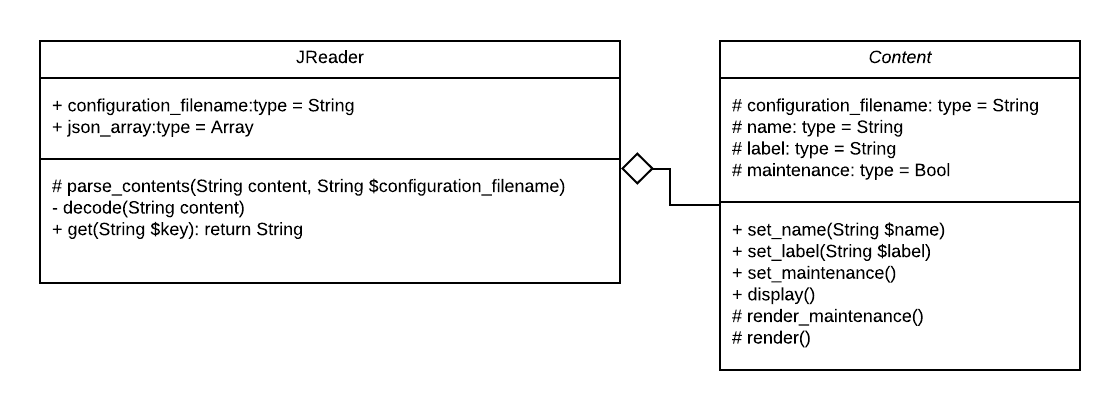
\includegraphics[width=1\textwidth]{content_uml_diagram}
    \caption{\Class{Content} class UML diagram describing its interaction with \Class{JReader}}%
    \label{fig:content_uml_diagram}
\end{figure}

\GSnote{}{Do you have a block-tree diagram that shows all of these relationships? Something like the one that gets generated when you run doxygen on C++ code}
\GOnote{}{We have included the UML diagram of Content class that way, since for an internal note it would be expected that the reader understands it. In case we turn it into a pubnote, then we will have no explain better the diagram. We found doxygen even more complicated.}
%-------------------------------------------------------------------------------

%-------------------------------------------------------------------------------
% 4 Analysis and Paper Phases  
% !TEX root = ANA-GENR-2018-01-INT1.tex
% Turn off some chktex warnings.
% chktex-file 1 chktex-file 8 chktex-file 46

%------------------------------------------------------------------------------
\section{Analysis and paper phases}%
\label{sec:Analysis_and_paper_phases}
%------------------------------------------------------------------------------

For many years ATLAS used FENCE to support the approval process of Papers, CONF and PUB notes.
At that time, the three types of documents and their related interfaces were considered as independent systems.
They had different creation interfaces, different search interfaces and different workflows, all starting from the Phase 1 of the pulication process, where the first draft is reviewed and approved.
Recently, Since CERN has stopped supporting SVN~\cite{svn}, many projects at CERN changed their version control software to Git~\cite{git} so the need of a new FENCE system that could interface with this technology emerged.
Thus, a new system called Analysis/Phase 0 was developed to communicate with GitLab~\cite{gitlab} through its API~\cite{rest_api}. It was also the opportunity to provide an interface to support and formalize the initial stages of a publication writing until a first draft is ready, the called Phase 0, before accessing the Paper, CONF or PUB note production process.
In this section, the way in which the software tools, mainly the FENCE framework, are used to achieve the Analysis/Phase 0 requirements is presented.
In \cref{fig:Glance_Papers_Phase0}, a screenshot of the main interface of the system is shown, where the user can have an overview of all the publication basic data and Phase 0 steps.
It is also possible to move forward the workflow triggering automatic messages that alert the responsible for the next step that they should perform an action in the system, giving them instructions.

\begin{figure}[htb]
  \centering
  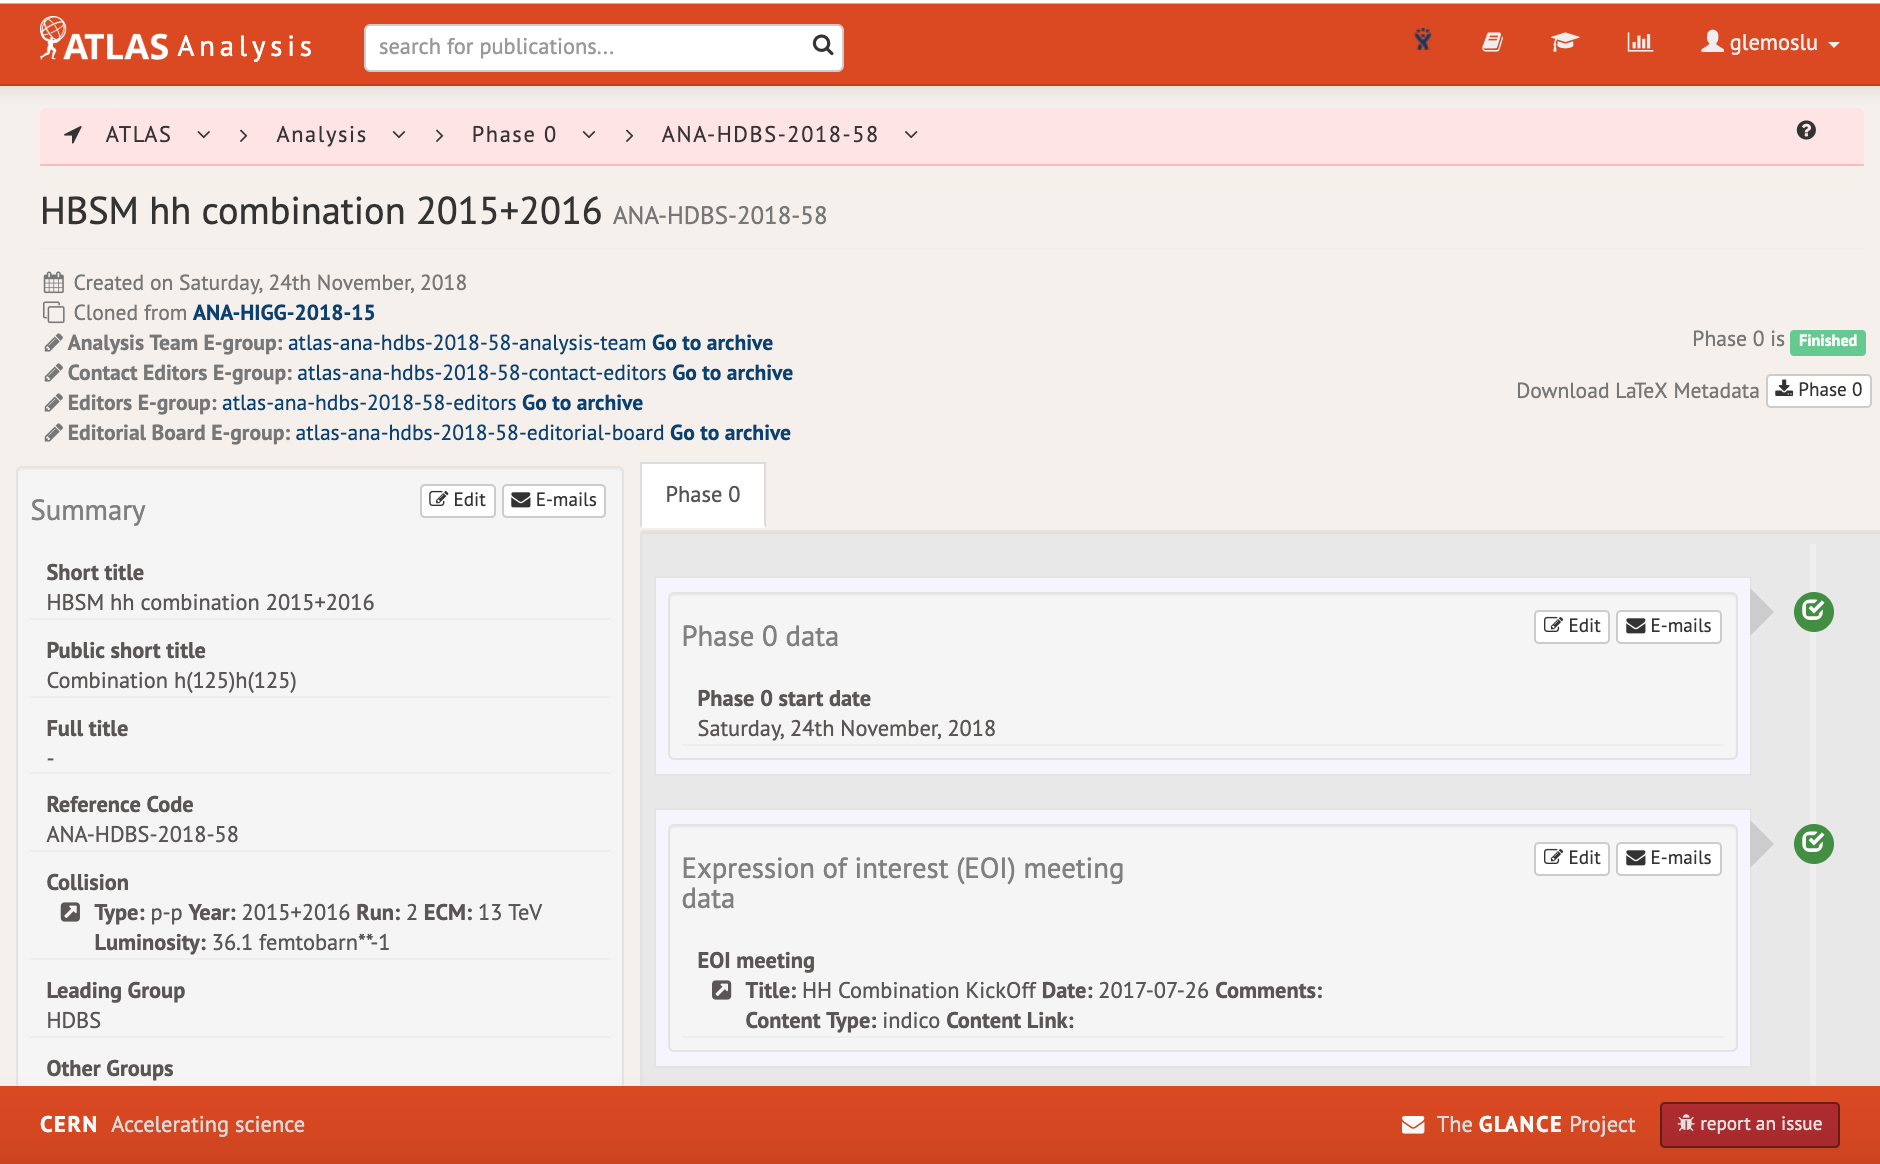
\includegraphics[width=0.9\textwidth]{figures/Glance_Papers_Phase0.png}
  \caption{Screenshot of the Analysis/Phase 0 system main interface. On the left panel, a summary of the most important metadata is shown such as titles, reference code, which is a unique reference to the publication, and collision type. On the right panel, Phase 0 related steps and metadata are shown.}%
  \label{fig:Glance_Papers_Phase0}
\end{figure}

Phase 0 is a common stage for Papers, CONF and PUB notes workflows, before Phase 1.
It stores some metadata divided into steps, e.g.\ meeting dates, comments, links, groups of people like Analysis Contacts and the target date for analysis finalisation, Editorial board members and meetings, approval sign-off dates.
Each of those metadata should be filled in a \GSnote{specific order}{Is the order documented in this note?}, \GSnote{by certain users}{Is that documented in this note? Who?} and trigger automatic emails or egroups~\cite{egroups} updates} along the process.

A real example is the Editorial Board request meeting and formation data step illustrated in \cref{fig:editorial_board_step}. The group convener is responsible for adding the Editorial Board request meeting title, date, comments and links. The Publication Committee Chair is responsible for appointing the Editorial Board members and fill the date that they were appointed. Once all those information are inputed in the system, the Publication Committee Chair can proceed to the next Phase 0 step using the green button. With the click of the button, the Editorial Board egroup is automatically formed with all its members and also, an email is sent informing them that they were appointed and should proceed the workflow in Analysis/Phase 0 system.

\begin{figure}[htb]
  \centering
  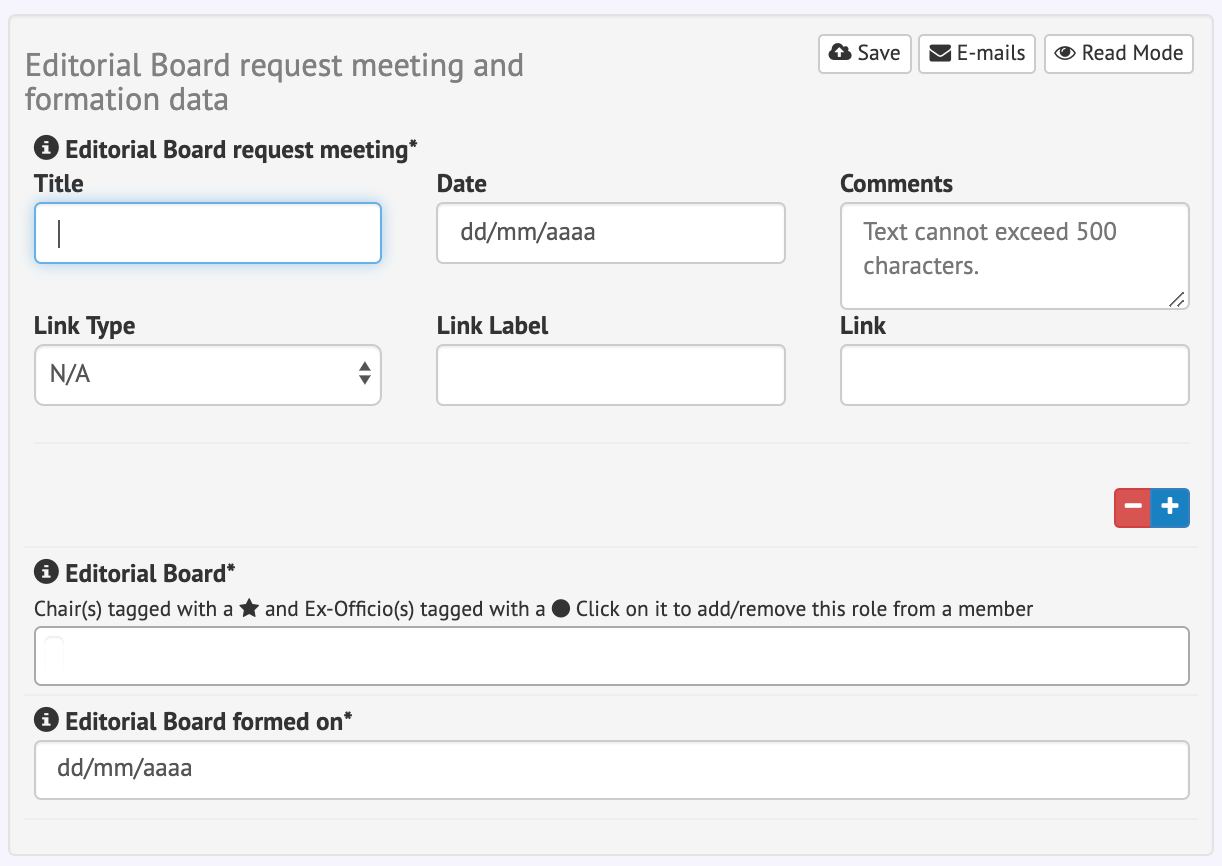
\includegraphics[width=0.9\textwidth]{figures/editorial_board_step.png}
  \caption{Screenshot of Editorial Board request meeting and formation data step in Analysis Phase 0 system.}%
  \label{fig:editorial_board_step}
\end{figure}

The main FENCE framework classes that allowed the development of those features are the \Class{Workflow}, \Class{Messenger}, \Class{EgroupManager} and \Class{User}.
Use is also made of many other classes and tools like the MBF (Models, Builder and Factories) infrastructure.
A brief explanation of the usage of each one is presented next.

%------------------------------------------------------------------------------
\subsection{\Class{Workflow} class}%
\label{sec:Workflow_class}

The \Class{Workflow} class was developed based on the concept of Directed Cyclic Graphs (DCG), that encompasses the relation between objects. In this context, objects are called nodes and the relation between them are called edges, being a directional flow. To represent this concept through a codified depiction, some classes were created.

The abstract \Class{Graph} class, whose code can be found in \cref{app:analysis:graph}, has a few simple implemented methods that allow the addition and deletion of nodes and edges.
The class that implements \Class{Graph} is called \Class{MapperGraph} and it stores nodes and edges inside a PHP data structure called \Structure{SplObjectStorage}, that, for this implementation, could better manage objects than associative arrays.
The usage of this data structure allowed the development of very simple methods to retrieve neighbour nodes or even edges given its origin and target node, which means retrieving a directional edge.

The \Class{Node} class defines methods to set and get data related to one node. The Edge class defines similar methods, but related to an edge. An example of data that can be added to an edge is an instance of the \Class{Action} class, having methods to set and get function callbacks, defining its arguments and being able to access its outputs.
More details about the \Class{Action} class implementation can be found in \cref{app:analysis:action}.

The \Class{Workflow} class, one of the most important classes of the Analysis/Phase 0 system since it is mainly characterised with Phase 0 steps with actions in between them, uses the Graph, Node, Edge and Action classes. It defines nodes as being Phase 0 steps, edges as being the relation between them and having actions being triggered, for example, sending automatic emails, updating egroups~\cite{egroups} and saving data in the Database.

The behaviour of the \Class{Workflow} class is controlled by a JSON file, following the FENCE pattern described in \cref{sec:Configuration_files_in_FENCE}.
This file defines all Phase 0 steps, having their identifiers and the inputs that should be rendered in each step, specifying their types, rules and permissions.
It also has the actions that can be triggered from one step with their function callback and the next state which the workflow should be moved to. An example is shown in the following piece of code:

\begin{lstlisting}
{
    "label" : "Analysis definition after EOI meeting",
    "identifier" : "analysis_definition",
    "inputs" : [
        {
            "label": "Main physics aim",
            "name": "main_physics_aim",
            "about": "",
            "type": "textarea",
            "rules": {
                "maxlength": 500
            },
            "edit": {
                "usergroups": [
                    "GROUP_CONVENER",
                    "SUBGROUP_CONVENER",
                    "PROJECT_LEADER"
                ]
            }
        }
    ],
    "actions" : [
        {
            "next_state" : "analysis_coordinators_selection",
            "callback": {
                "class": "Atlas\\Analysis\\Analysis\\WorkflowActions",
                "method": "proceed"
            },
            "usergroups": [
                "GROUP_CONVENER",
                "SUBGROUP_CONVENER",
                "PROJECT_LEADER"
            ]
        }
    ],
    "notifications" : [
        {
            "template" : "EOI_MEETING_RESULTS",
            "task": "proceed",
            "deploy_on": "taskTriggers"
 },
        {
            "template" : "ANALYSIS_COORDINATOR_REQUEST",
            "task": "proceed",
            "deploy_on": "taskTriggers"
        }
    ]
}
\end{lstlisting}

The example is a part of the JSON file setting the step for analysis definition
after the Expression of Interest (EOI) meeting.
First, the identifier of the step is set as analysis$\_$definition.
Then, the main physics aim input is defined with its label, identifier, instructions (if any), type (in this case, a text box), its rule of maximum 500 characters and also the editor permissions. After, the actions are defined with their function callback path and permissions.
The callback can instantiate any other class like \Class{Messenger}, to send automatic emails or \Class{EgroupManager} to update egroups.
Finally, email notifications to be sent are defined through templates, specifying when they will be triggered.

%------------------------------------------------------------------------------
\subsection{Messenger class}%
\label{sec:Messenger_class}

The \Class{Messenger} class is used by the \Class{Workflow} class to send automatic emails and also to allow users to edit email templates. As explained before, the JSON file used by the \Class{Workflow} class defines email template names to be triggered by an action.
These templates and their variables are stored in the database in two JSON files.
The first one contains all the templates with variables to be substituted and the second contains the variables' identifiers and the methods used to substitute them in the templates before sending the email.
Using another class called \Class{DBJReader}, the \Class{Messenger} class can read these JSON files from the database.
Then, it can either get the templates and show them in the interface so the users can edit them or parse the variables and send an email.
In the first case, the changes performed in the templates are saved again in the database, but this time using the \Class{DBJWriter} class.
In the second case, \Class{Messenger} class will substitute all the variables in the template and use the \Class{Mailer} class to trigger the email to the correct recipient.
A summary of this infrastructure can be found in \cref{fig:Messenger_class}.

\begin{figure}[htb]
  \centering
  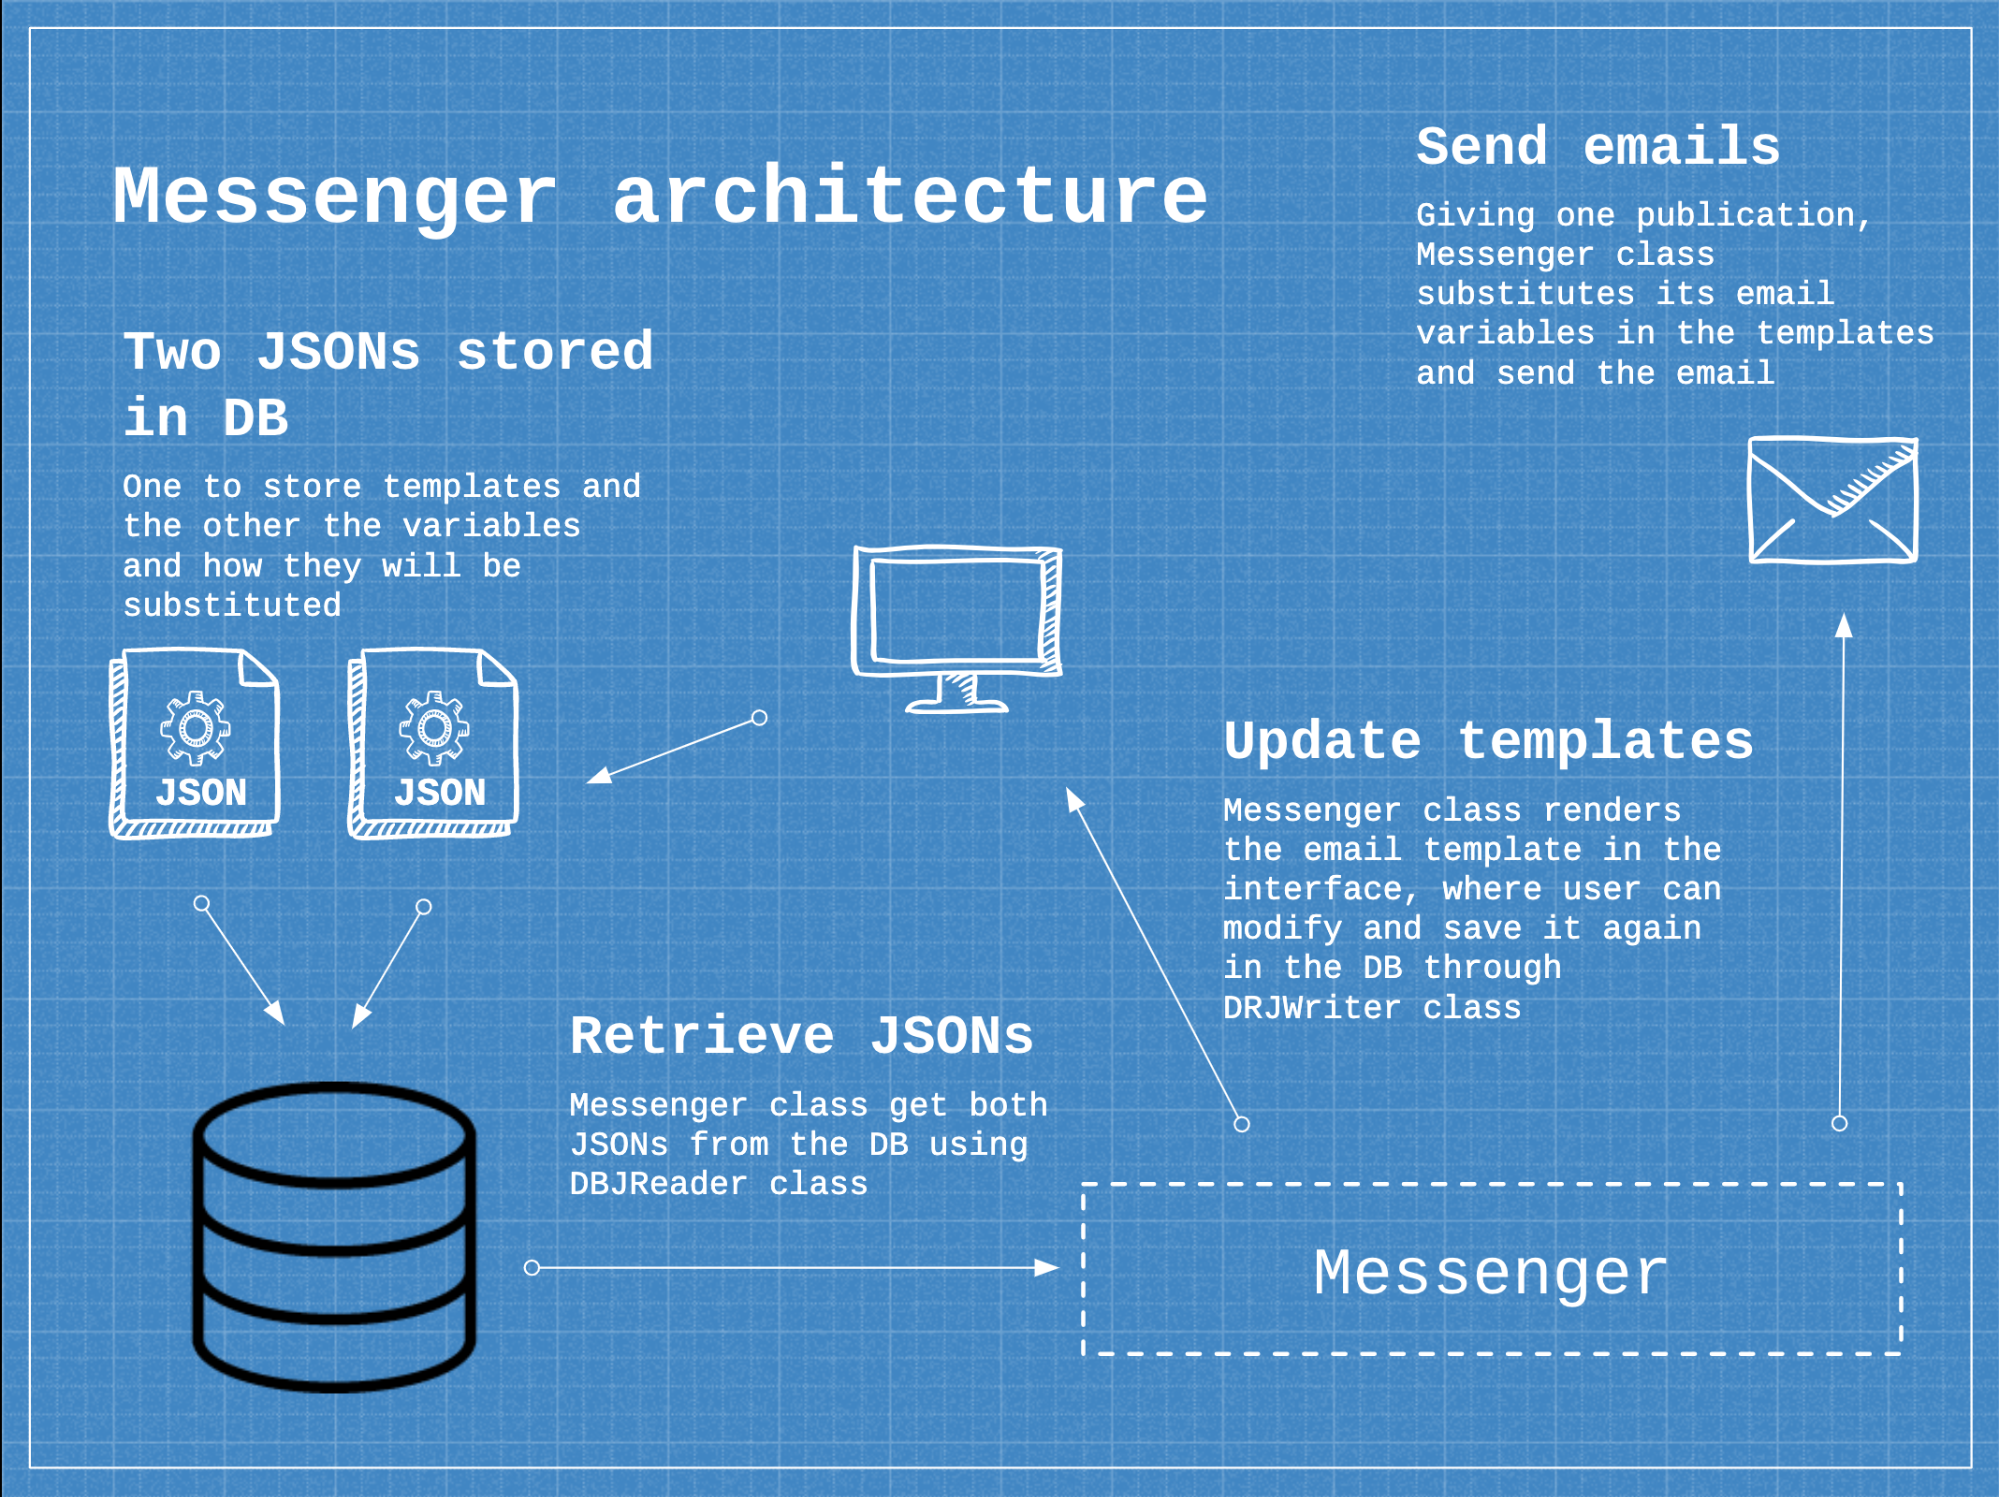
\includegraphics[width=0.9\textwidth]{Messenger_class}
  \caption{Summary of the \Class{Messenger} class infrastructure. The two JSON files related to the \Class{Messenger} class are stored in the database. The class retrieves them using the \Class{DBJReader} class. \Class{Messenger} can either use the FENCE \Class{Mailer} class to trigger emails or render emails templates so users can edit them though the Analysis/Phase 0 system interface, represented by the computer. After the user edition, the JSON email templates are saved again th the database using the \Class{DBJWriter} class.}%
  \label{fig:Messenger_class}
\end{figure}

In \cref{fig:email_template_editing} the interface that allows the editing and re-sending of an email template is shown. It is possible to set the recipients (To, Cc and Bcc), an additional email address not in the default list, the subject and the content of the email.
Those last two can have variables to be substituted according to the publication.

\begin{figure}[htb]
  \centering
  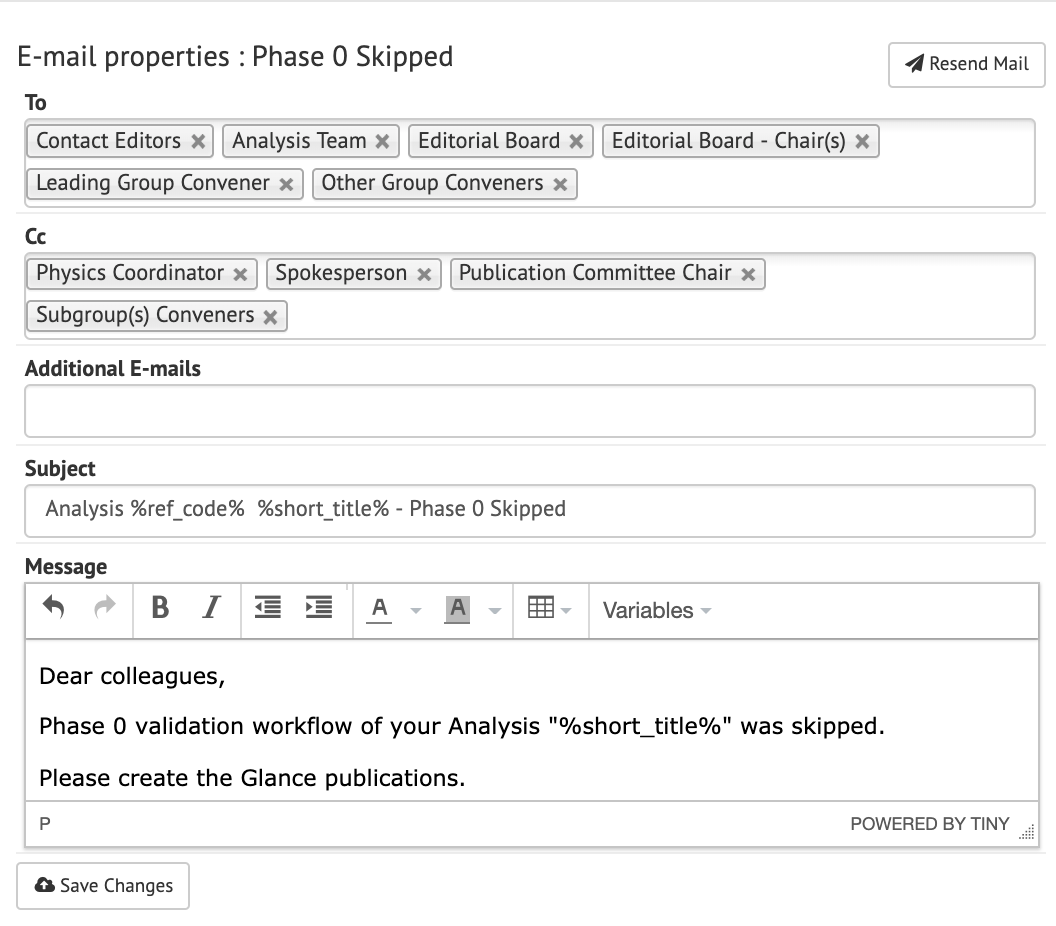
\includegraphics[width=0.9\textwidth]{email_template_editing}
  \caption{Interface for email template editing.}%
  \label{fig:email_template_editing}
\end{figure}


%------------------------------------------------------------------------------
\subsection{\Class{EgroupManager} class}%
\label{sec:EgroupManager_class}

The \Class{EgroupManager} class is similar to the \Class{Messenger} class since it also gets a template from a JSON file and substitutes variables.
The difference is that the templates are not related to emails, but egroup configurations.
Also, it does not allow users to edit the templates from the interface since they contain many technical details.

The \Class{EgroupManager} class first uses another FENCE class to get the templates from the JSON file called \File{JReader}, designed to parse JSON files and save them in an object.
After getting the JSON templates, \Class{EgroupManager} parses it substituting all the variables.

One example that can be found in \cref{app:analysis:egroupmanager} is the Analysis Team egroup created when there is a new Analysis/Phase 0 entry.
The template contains its identification, the name of the egroup with already one variable to be substituted, the Analysis/Phase 0 reference code.
It also defines a topic, administrator egroup and posting exceptions, some mandatory parameters to create an egroup through its API\@.
The members of the egroup will then be substituted by the Analysis team members when the \Class{EgroupManager} class parses the variables.

Having the template parsed, the \Class{EgroupManager} class uses the FENCE \Class{EgroupSOAPHandler} class to communicate with the egroups API\@.
To do so, it first makes an authentication and, using the methods available in the SOAP WebServices~\cite{egroups}, it can create, update or delete egroups.


%------------------------------------------------------------------------------
\subsection{\Class{User} class}%
\label{sec:User_class}

The main purpose of the \Class{User} class is to define an object that stores information concerning the logged in CERN member, for instance, his or her CERN CCID, first and last name, egroups and others attributes. Besides that, it defines specific methods, to facilitate the access control among the interface.
In \cref{app:analysis:userauthorise}, we have two examples of the above mentioned methods.
These are used to check user authorization:
\Class{is$\_$expert()} checks if the user is member of \enquote{fence-developers} egroup, which is composed by the project developers. % chktex 36
The method \Class{Permission($\$$permission)} accepts a permission to be checked as an argument and verifies if it is among the user permissions inventory. % chktex 36
Moreover, when an extension of \Class{User} is created, extra methods are appended to \Class{User} to provide specific \textit{utils} for a context.
This way, every system has its own \Class{User} class extending the FENCE core \Class{User} class.
This is the case for \Class{Analysis}, which has many specific methods used to grant edit permissions and control users access.
Furthermore, \Class{Analysis} was implemented using the concept of configuration files, described in \cref{sec:Configuration_files_in_FENCE}.
These files provide multiple properties that set access control and edit permissions on Analysis systems. This is mainly achieved in two ways. General access control is set using CERN egroups, or FENCE user groups, such as experts, administrators and many others.
In this case, \Class{User} class verifies the clearance by comparing the user egroups and user groups to the ones contained on its object.
The other way concerns inputs edit permissions and uses analysis specific roles to do so.
These roles are keys mapped to methods in \Class{User} class that check if the member is supposed to have edit permission on that specific field.
An example is shown next:

\begin{lstlisting}
"pub_short_title": {
    "label": "Public short title",
    "sublabel": "Plain text, no LaTeX",
    "type": "textarea",
    "rules": {
        "maxlength": 1000,
        "character_not_allowed": ["\\", "$"]
    },
    "analysis_roles": [
            "GROUP_CONVENER",
            "SUBGROUP_CONVENER",
            "PROJECT_LEADER"
    ]
}
\end{lstlisting}

Taking the \texttt{GROUP\_CONVENER} role as an example, it uses the following method to grant permission to edit the Public short title field:

\begin{lstlisting}
public function is_subgroup_convener($publication_id = null)
{
        if ($publication_id === null) return false;
        foreach ($this->subgroup_convener_publications as $line => $row) {
                if (strpos($row['PUB_LIST'], strval($publication_id)) !== FALSE) return true;
        }
        return false;
}
\end{lstlisting}


%------------------------------------------------------------------------------
\subsection{MBF (Models, Builder and Factories) infrastructure}%
\label{sec:MBF_Models_Builder_and_Factories_infrastructure}

Models, Builders and Factories are all individually heavily used software design patterns.
However, their combined usage is a particular feature of FENCE framework.
The main goal of these development standards is to create a wrapper to store complex objects and facilitate the construction of these on different contexts, working as a SQL query builder.
For instance, it would be possible to pass an actual SQL Query every time information from the database is needed.
It is, however, much more convenient to just call a class that handles the queries and presents to the user the needed object.
The desired behaviour described above is exactly how the MBF infrastructure works.
On FENCE classes, objects are constructed simply by instantiating specific factories classes.
These classes extend the core \Class{Factory} class, which sets the whole engineering that connects to the database and assembles objects.
Whenever a specific new object needs to be created, a group of three files are needed: the Factory, the Builder and the Model files.
Models are classes that serve as an oriented object representation of the information. They define several sets and get methods that handle specific properties of the object. These models are used in Builders, where the actual query is set and database columns are associated to a model set method. Finally, a Factory calls its corresponding Builder and also contains an inventory, which may be empty, of other Factories that are related to this object.

The \Class{Workflow}, \Class{Messenger}, \Class{EgroupManager} and \Class{User} classes, along with the MBF infrastructure made possible the development of the Analysis/Phase 0 system workflow, well represented by \cref{fig:Glance_Papers_Phase0}.
However, they do not include the GitLab Integration, a key feature of the system, that will be explained in detail in the next sections.

\GSnote{}{More example code, and charts/trees would help to clarify a lot of this. There's a lot of text that's very dense and hard to parse without more figures.}

%-------------------------------------------------------------------------------

%-------------------------------------------------------------------------------
% 5 PO-Gitlab and CI tools
% !TEX root = ANA-GENR-2018-01-INT1.tex
% Turn off some chktex warnings.
% chktex-file 1 chktex-file 8 chktex-file 46

%------------------------------------------------------------------------------
\section{PO-GitLab and CI tools}%
\label{sec:PO-Gitlab_and_CI_tools}
%------------------------------------------------------------------------------

The Physics Office GitLab \GSnote{project}{Is it a project or a group?} (\pogitlab) aims to simplify the creation,
\IBnote{editing and publication}{I think we have to separate more clearly the editing and publicatiuon phases in the note} process of ATLAS documents (papers, CONF notes, PUB notes and internal notes) by using the tools provided by the CERN GitLab system.
The previous publication workflow consisted of a heavy e-mail communication between ATLAS editors and the Physics Office in order to ensure that ATLAS rules were being followed, before being able to submit the desired paper to arXiv or to the journal of choice.
This approach led, usually, to modifications done by different parties (officers and editors), which were sometimes not properly implemented \GSnote{by the other party}{delete}.
This slowed down the publication process due to small details, which, with a different approach can easily be avoided.
There are three main areas modified by the PO-GitLab approach with the goal of simplifying this process. These areas are the automatic creation of the document GitLab projects (Git repositories in a centralised way), the real-time verification by the GitLab Continuous Integration (CI) tools of the documents being written and the automatic processing of the document to ensure an accurate publication process. These areas are described in this section.


%------------------------------------------------------------------------------
\subsection{Automatic document creation}%
\label{sec:Automatic_document_creation}

First, a centralised area controlled by ATLAS Physics Office needed to be designed.
The control is key in order to allow Physics Office to maintain quality control over the document being accepted for publication.

A basic structure is already set in GitLab to store the groups related to an analysis.
The main GitLab group is called \texttt{atlas-physics-office} and it contains many subgroups. Each of these subgroups belongs to a leading group, \GSnote{for example: Higgs, Exotics, SUSY etc., see \cref{fig:Gitlab_repository}}{Use this to callback to an earlier example with the ANA-HDBS-2018-58 -- by explaining what would get created as part of Phase 0/Phase 1/etc... that you showed in~\cref{fig:Glance_Papers_Phase0}}.

Having this structure defined, it is possible to automatically create documents through FENCE, thanks to the communication between the framework and the GitLab API in the so called FENCE and Gitlab integration.
This is explained in more detail in \cref{sec:FENCE_and_Gitlab_integration}.
This amortisation relies on file templates that have their variables substituted according to the related publication.
This way, all the created repositories contain the default documents correctly formatted to start writing a paper, CONF, PUB or an internal note.
The repository is also configured with all the needed branches,
\IBnote{labels}{The word labels is used for various tings in this document. We should clarify the nomenclature.} and also placed in the correct GitLab \GSnote{group}{group? See Ian's comment as well applies here}.


%------------------------------------------------------------------------------
\subsection{Real-time check with GitLab’s CI}%
\label{sec:Real-time_check_with GitLabs_CI}

GitLab CI tools are designed to \GSnote{execute a set of automatic tasks}{automatically execute a set of tasks} every time a new modification is introduced in the document (i.e.\ a new commit is pushed to the document repository).
The approach from the Physics Office was to develop a package that is able to run different jobs on a given document, verifying distinct aspects, which are executed by the \pogitlab Python package~\cite{pogitlab-repo}.
Given the modularity of the system, new and/or more complex tasks can me added, ensuring scalability.

\GSnote{}{Here is a good time to show code examples of different calls you can make on a given document to show how the command-line interface for the Python package works...}

GitLab’s CI \GSnote{works through pipelines}{is organized using pipelines}. Each time a new commit is pushed to the repository, a pipeline is triggered.
A pipeline is a set of jobs grouped in stages. All the jobs in the same stage are executed in parallel while each stage is only executed once the previous one has \GSnote{finished}{Just a note that there's no requirement for the stage to have finished successfully... can also only execute if the previous stage failed, for example}.
The \GSnote{real-time verifications}{checks} are performed in \GSnote{most of the branches}{which branches? what pattern?} of the project and they are called \enquote{edit-pipelines}.
There are \GSnote{additional pipelines that are used when a paper is ready for submission}{which branches? when are these run?} to the arXiv and a journal. These are referred to as \enquote{submit-pipelines}.

\begin{figure}[htb]
  \centering
  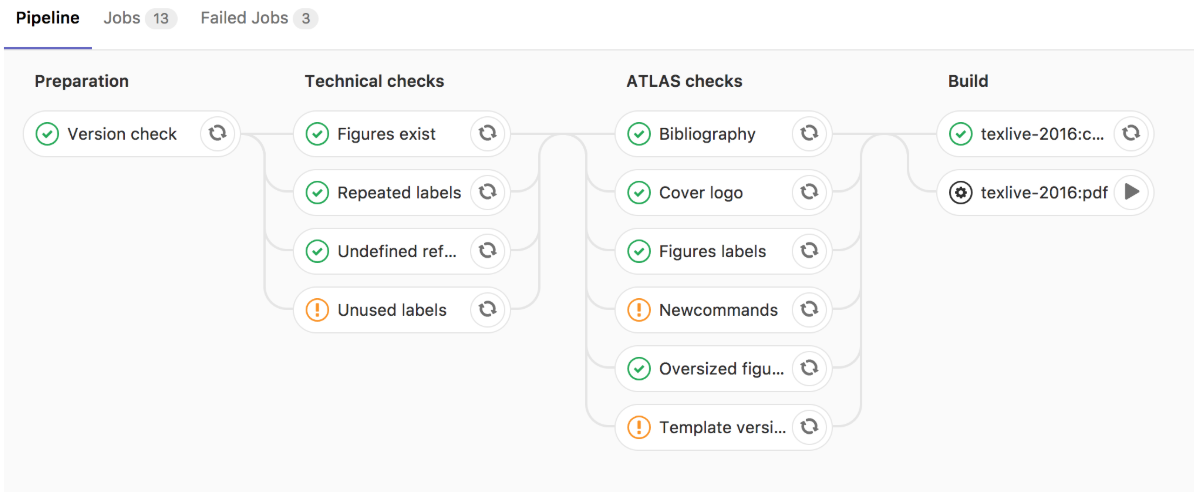
\includegraphics[width=0.9\textwidth]{editing_pipelines_1}
  \caption{Screenshot of the edit-pipelines. \GSnote{}{Expand caption. Explain that there are 4 stages in this image, with the preparation stage checking the version of the po-gitlab package, the second stage is ..., the third stage is ..., etc... This is explained in more detail in the note, so an abridged summary here is good.}}%
  \label{fig:edit-pipelines}
\end{figure}

\Cref{fig:edit-pipelines} presents an example of the edit-pipelines that consist of the following set of stages:
\begin{itemize}
\item \textbf{Preparation}: It consist of only one job that checks the current version of the \pogitlab package.

\item \textbf{Technical checks}: This stage includes checks related to \LaTeX: % chktex 13
  \begin{itemize}
  \item Figures exist: check if all figures used in the document are present in the repository or if any is missing.
  \item Files exist: check if all the \File{tex} files included in the document are present.
  \item Repeated commands: checks for repeated user-defined commands.
    It is not wise to use the same command for different purposes and can be an issue when generating captions for figures and tables for the ATLAS public pages.
  \item Repeated labels: checks for duplicate labels in all \File{tex} files.
  \item Undefined references: checks for undefined references.
  \item Unused labels: warnings of a \LaTeX\ label which has been defined but not used.
    Although this is not an issue it might point to something not being properly referenced.
  \end{itemize}

\item \textbf{ATLAS checks}: These are checks related to ATLAS rules and style:
  \begin{itemize}
  \item Bibliography: checks that the bibliography files are included.
  \item Cover logo: checks that the proper logo is being used in the ATLAS template.
  \item Figures labels: checks the ATLAS labels (e.g.\ \enquote{ATLAS Internal}) in the legends of figures depending on the type of document. \Cref{tab:labels} shows the different labels which are allowed and not allowed in different files.
  \item Oversized figures: checks for figures larger than \SI{2}{\mega\byte}.
  \item Preprint ID\@: checks that the preprint ID is included in the document.
  \item Template version: checks that the version of the ATLAS \LaTeX\ template is the latest one available.
  \item Title and Abstract: checks that no user-defined commands (i.e.\ non-\LaTeX\ commands) are being used in the title and in the abstract.
  \end{itemize}

\item \textbf{Build}: this stage builds the document itself. The PDF file of the document is not usually \GSnote{saved}{stored as an artifact} to avoid \GSnote{increase in size of the repository}{You can always store as an artifact, but mark it to expire in 24h... so this is a weird justification}.
However, a manual job (only run when \GSnote{requested}{who requests?}) can build the document and save the PDF file as an artifact for \GSnote{the}{a} user to download.
\end{itemize}

\begin{table}[htb]
  \centering
  \begin{tabular}{lll}\toprule
    Document type & Preliminary label & Internal label \\
    \midrule
    PAPER & Not allowed & Not allowed \\
    BOOK & Not allowed & Not allowed \\
    CONF & Allowed & Not allowed \\
    PUB & Allowed & Not allowed \\
    NOTE & Allowed & Allowed \\
    \bottomrule
  \end{tabular}
  \caption{Labels in legends that are allowed and not allowed in figures depending on the document type.
  The files and figures exist checks are needed because it is rather common to forget committing a new file or figure. \GSnote{}{I don't understand the caption. Please rephrase/clarify.}}%
  \label{tab:labels}
\end{table}

%------------------------------------------------------------------------------
\subsection{Paper submission}%
\label{sec:Paper_submission}

\GSnote{The GitLab’s CI}{The CI} also produces the required files for paper submission, using dedicated pipelines, similar to the editing ones.
These are referred to as \texttt{submit-pipelines} here.
A protected Git branch, named \texttt{PO-ready}, is created by default at the time of the setup of the paper repository.
When a paper is ready for submission, an editor should create a \enquote{Merge Request}
from the \texttt{Master} to the \texttt{PO-ready} branch.
When this request is accepted by a Physics Office officer, the paper submission pipelines are triggered.
In addition, any \IBnote{branch}{also tag?} created with a name of the form \texttt{PO-*} triggers the paper submission pipelines.
These pipelines have the previously described tests, but after at the build stage a flattening of the LaTeX document happens, with the following actions:

\begin{enumerate}
\item all the source files are merged into a single \LaTeX\ source file;
\item all the comments in the \LaTeX\ source file are removed;
\item all the figures are renamed following the convention required by the APS journals;
\item any directory structure is removed.
\end{enumerate}
The various actions are shown in \cref{fig:submit-pipelines}.

Furthermore, tarballs suitable for submission to arXiv and APS journals are created using \TeX{}Live \GSnote{2016 and 2017}{First time mentioning the version years.. need a section explaining when/why you pick specific versions to support}, respectively, and a tarball with the required files for the public webpage with plots and tables is created. These tarballs are created as GitLab artifacts and can be downloaded by the members of the Physics Office and editors. In the submission tarballs, the auxiliary material (figures and tables not for submission) are not included.

\begin{figure}[htb]
  \centering
  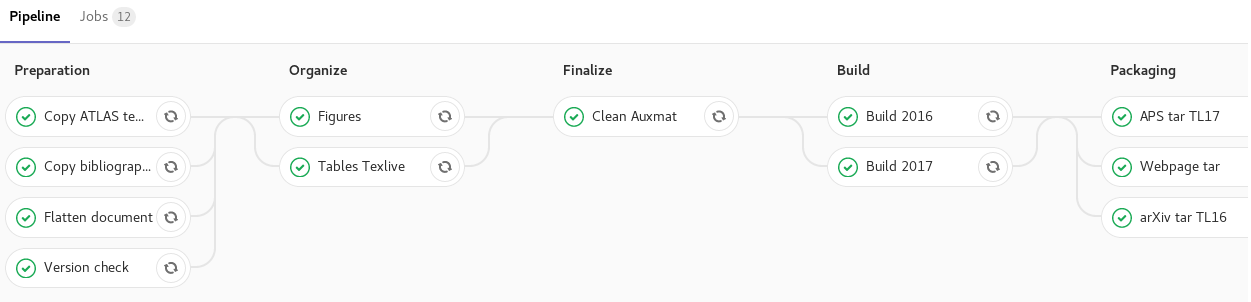
\includegraphics[width=0.9\textwidth]{editing_pipelines_2}
  \caption{Screenshot of submit-pipelines. \GSnote{}{Please expand caption more... you don't have any details of these stages in the text like you did with the edit-pipeline}}%
  \label{fig:submit-pipelines}
\end{figure}



%-------------------------------------------------------------------------------

%-------------------------------------------------------------------------------
% 6 FENCE and Gitlab integration
% !TEX root = ANA-GENR-2018-01-INT1.tex
% Turn off some chktex warnings.
% chktex-file 1 chktex-file 8 chktex-file 46

%------------------------------------------------------------------------------
\section{FENCE and GitLab integration}%
\label{sec:FENCE_and_Gitlab_integration}
%------------------------------------------------------------------------------

As already mentioned before, the FENCE Analysis Phase 0 project originated from the requirement to have an automatic creation of Gitlab repositories for each Analysis or publication. So Phase 0 interface has some features that triggers the communication with Gitlab. The integration was already mentioned in section 5.1, but it will be described in details in this section.

%------------------------------------------------------------------------------
\subsection{GitLab structure to organise Analysis groups and repositories}%
\label{sec:Gitlab_structure_to_organise_Analysis_groups_and_repositories}

Analysis groups and repositories are created in GitLab under the atlas-physics-office group. Each Leading Physics, Combined Performances group or a SyStem Detector/Activity coordination is labelled as a category with four letters in FENCE Analysis systems.
For example, the leading TOP Quark physics group is \texttt{TOPQ} while the Electron/Gamma combined Performance group is \texttt{EGAM}. The ID of a Phase 0 FENCE entry is therefore labelled: \texttt{ANA-GROUP-YEAR-NN} where GROUP can be \texttt{TOPQ}, \texttt{HIGG} or \texttt{EGAM}, for example.
\texttt{YEAR} is the year when the document was created and \texttt{NN} is a two digit number.
For instance, ANA-SUSY-2019-04 for the 4th ANAlysis FENCE entry created in the SUSY group in 2019.
                    
An analysis group may evolve into a Paper, a CONF or a PUB note. The IDs of those documents are therefore respectively \texttt{GROUP-YEAR-NN}, \texttt{CONF-GROUP-YEAR-NN} or \texttt{PUB-GROUP-YEAR-NN}.
This naming convention preserves the backward compatibility with the different entries used for each type of document before Phase 0 creation.

Contrarily, in PO-Gitlab, the documents IDs are more logical and are labelled: \texttt{ANA-GROUP-YEAR-NN-INTn} in the case of an internal note,
\texttt{ANA-GROUP-YEAR-NN-PAPER} in case of a paper,
\texttt{ANA-GROUP-YEAR-NN-CONF} for a CONF note,
\texttt{ANA-GROUP-YEAR-NN-PUB} for a PUB note.
For example, in the Higgs category, for a given Phase 0 Analysis entry \texttt{ANA-HIGG-2017-08},
\pogitlab will host \texttt{ANA-HIGG-2017-08-INT1,2..n, ANA-HIGG-2017-08-PAPER, ANA-HIGG-2017-08-CONF, ANA-HIGG-2017-08-PUB}.
Each repository is connected to the appropriate FENCE interface.
This can be seen in \cref{fig:Gitlab_repository} where the \gitlab interface for the atlas-physics-office subgroups and repositories is shown.
\texttt{ANA-HIGG-2017-08}, a subgroup of HIGG, in fact contains one paper and one internal note repository, namely \texttt{ANA-HIGG-2017-08-PAPER} and \texttt{ANA-HIGG-2017-08-INT1}.

\begin{figure}[htb]
  \centering
  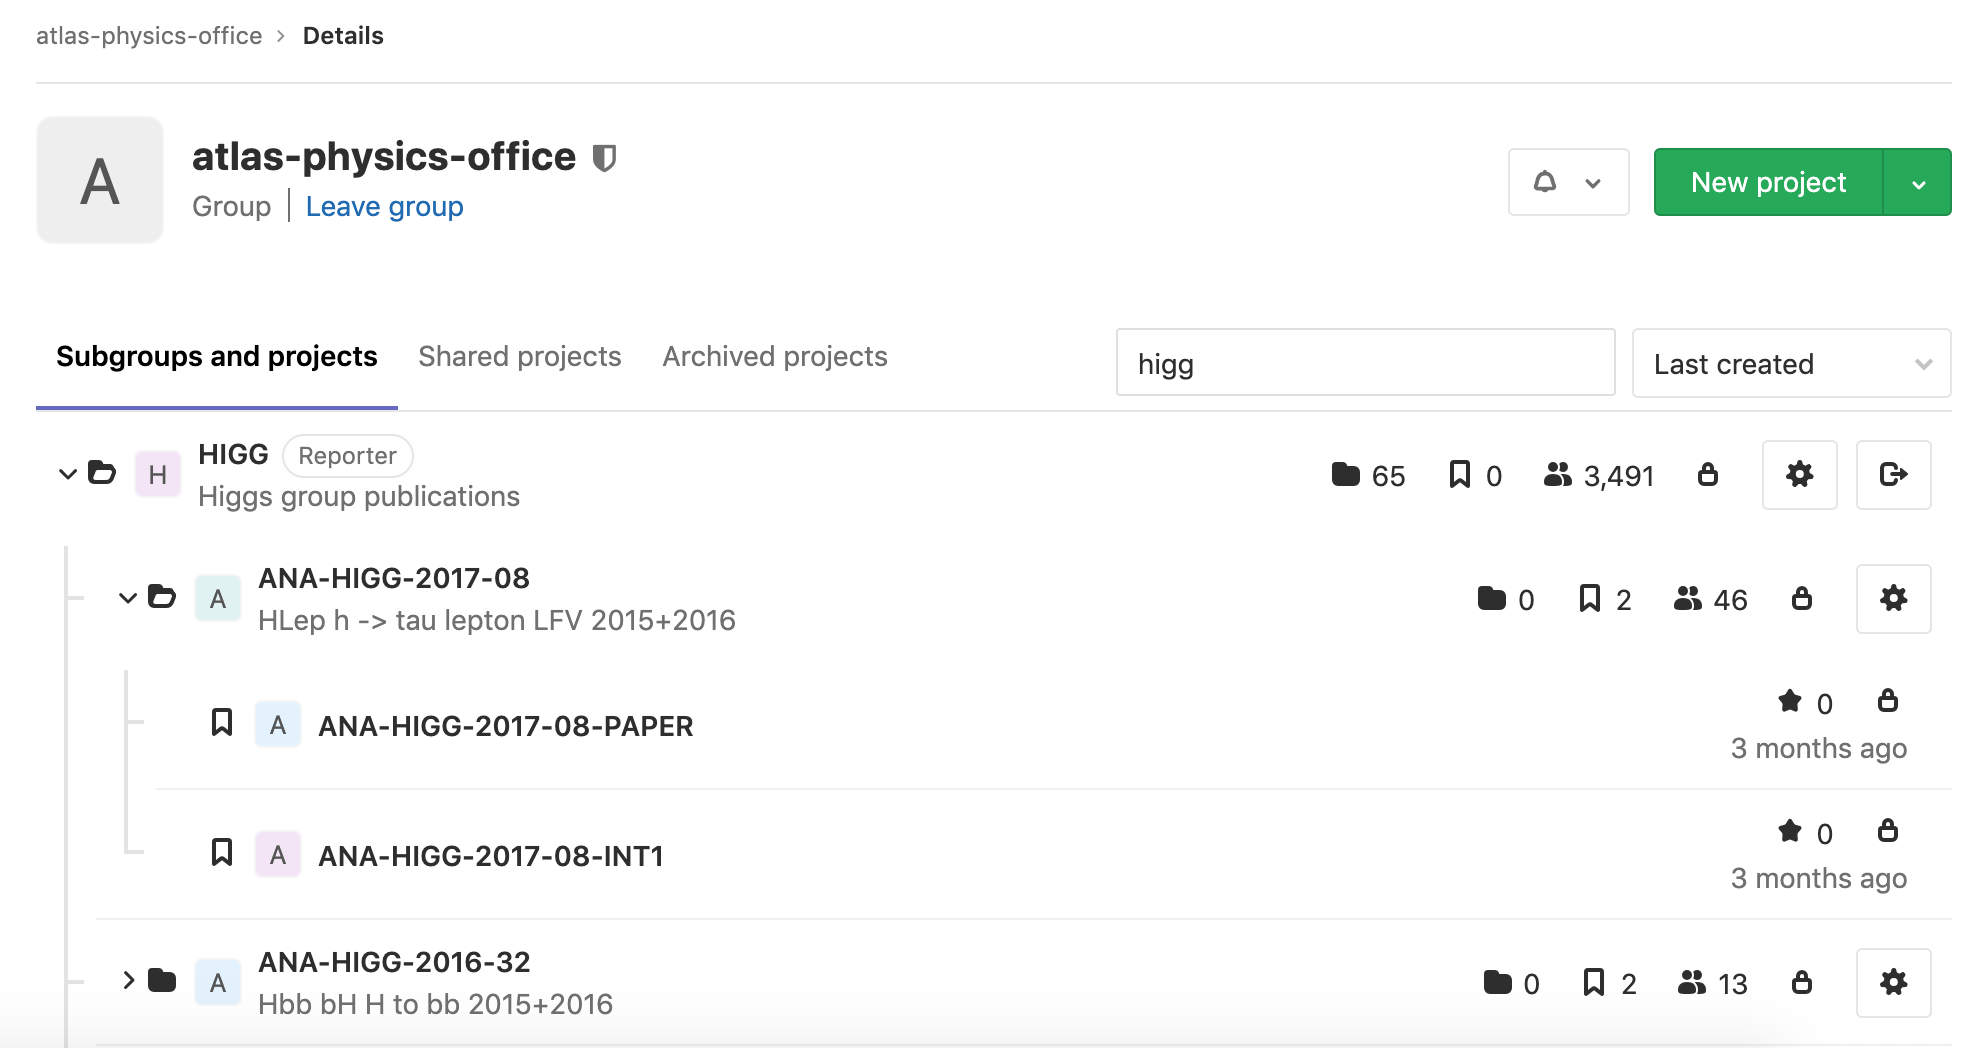
\includegraphics[width=0.9\textwidth]{Gitlab_repository}
  \caption{Screenshot of a substructure of the HIGG Gitlab repository.}%
  \label{fig:Gitlab_repository}
\end{figure}

%------------------------------------------------------------------------------
\subsection{Middleware between FENCE and Gitlab REST API}%
\label{sec:Middleware_between_FENCE_and_Gitlab_REST_API}

A set of classes were created with the aim to make the usage of the \gitlab API easier among the FENCE systems, but is actually mainly used by the Analysis systems within the Analysis Gitlab integration.
Through the main class, called \Class{Gitlab}, it is possible to handle all the basic operations offered by the API\@: create, get and customise settings for projects, groups, branches, handle commits and many other actions defined and explained in the Gitlab REST API documentation~\cite{rest_api}.

Each API endpoint can be accessed by one of the following HTTP methods: GET, POST, DELETE and PUT\@.
The FENCE Gitlab class uses them through methods detailed in \cref{sec:app7}.
Each of those methods make a call to \Class{execMethod}, in \cref{sec:app8}, that configures the endpoint using the PHP CURL methods~\cite{php_curl} and executes one of the HTTP methods, returning the REST API answer, that can be a JSON file with metadata, or just a success, or an error message.

The metadata returned by the \Class{execMethod} is then used to populate the attributes of many classes representing some \gitlab elements like: 
\texttt{Branch, File, Commit, Project, Group, Label} and \texttt{Member}.
These can be then manipulated by any FENCE system.

An example is the creation of a paper repository.
The \Class{createProject} method (see \cref{sec:app9}) is called having the project name as the first argument (or even an instance of the \Class{Project} class) and project parameters as the second argument like path, namespace, default branch, description and others.
The method calls the POST method mentioned above and stores the new repository metadata in a FENCE \Class{Project} object, which can be used for further manipulations.


%------------------------------------------------------------------------------
\subsection{FENCE-Gitlab Integration}%
\label{sec:FENCE-Gitlab_Integration}
The first interaction between FENCE and Gitlab happens when a Phase 0 entry is created. A group with its reference code is automatically formed containing the first internal note repository. The content of this repository’s first commit is obtained from a source repository, a package containing file templates called atlaslatex. FENCE is responsible of substituting all the necessary variables in all the file templates according to the metadata inserted when creating the entry in the system. After the commit, FENCE automatically un-protects the master branch, creates the protected PO-ready branch and also creates PO-Publication label. The last step is to set the developer permission to the Analysis Team egroup using LDAP synchronisation.
                    
Another FENCE and Gitlab integration process is executed when Phase 0 is finished or it is skipped, proceeding to Paper, CONF or PUB note Phase 1. FENCE automatically creates an internal note repository setting all the configuration needed. It is also possible to append one or more additional internal note repositories at any time. The creation of configuration of the repositories holding the document is done without any input from the editor’s side allowing for a quick process. 

FENCE and Gitlab also interact while handling the author list of a publication. Creating the author list at first circulation will trigger a request for the existence of the Gitlab repository associated to the publication through the Gitlab API\@.
In a first transition period, if the repository did not exist, the author list would have been stored on AFS file system, that is now deprecated.
Nowadays a \gitlab repository associated to the paper is a mandatory prerequisite, and to force the user to use it, FENCE will not allow the creation of the author list until the repository, if missing, is created.

If the repository is set up, the act of clicking on the button labeled as “Create and push to Gitlab”, see \cref{fig:paper_authorlist_section}, after creating the author list bounded to its reference date on all the different formats (\File{xml}, \File{tex} and others), starts a dialog among the two platforms, FENCE and \gitlab, to correctly push the files through the \gitlab API add method.
On first circulation, new files are added to \gitlab, while on following circulations, the files, as they already exist, are pushed through the update method.

\begin{figure}[htb]
  \centering
  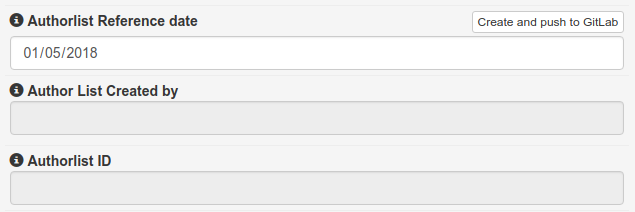
\includegraphics[width=0.9\textwidth]{paper_authorlist_section}
  \caption{A view of a paper's author list section: on first circulation,
  the \enquote{Create and push to GitLab} button generates the author list and triggers the push action on the GitLab repository.
  The button will change its label on following phases to \enquote{Generate and push to GitLab}.}%
  \label{fig:paper_authorlist_section}
\end{figure}

Another interaction is needed to avoid two types of errors that will result in a blocker operation: trying to update a file that does not exist, or adding a file that is already in the repository. Through the Gitlab API FENCE, it is possible to check the status of a file before committing to avoid these two kind of errors. This verification is important because users could accidentally have renamed/deleted/moved one of these files without Fence being able to record these kind of activities.
%-------------------------------------------------------------------------------

%-------------------------------------------------------------------------------
% 7 Author lists, Acknowledgements and Proof Checker
\section{Authorlists Acknowledgements and ProofChecker}
\label{sec:Authorlists_Acknowledgements_and_ProofChecker}

\subsection{Author lists and acknowledgments files}
\label{sec:Author_lists_and_acknowledgments_files}

Both types of files, author list and acknowledgements, are built using FENCE framework, see Fig.~\ref{fig:authorlist_interface}, and automatically pushed into the appropriate Gitlab repository, thanks to the FENCE Gitlab integration (chapter 6.3). Their implementation into the Paper is straightforward for a future submission to the journals. FENCE provides an elegant way to retrieve the needed information from the database (see chapter 4.5 MBF infrastructure) and build all the needed files.
 
The Author lists XML file is composed by three main blocks:
\begin{itemize}
\item Header: store paper main information (\ref{sec:app10})
\item Institutes: list of institutes and their references (\ref{sec:app11})
\item Authors: list of authors for this author list with their information (\ref{sec:app12})
\end{itemize}
 
XML file is the one used as a “role” since it contains all the information needed to build the other files. It is the first one to be generated and a backup version of the first release of the author list is stored.
 
The acknowledgment TEX file is built using a standard template and it is filled using the FENCE framework to retrieve the needed information about the ATLAS Founding Agencies.

\begin{figure}[ht!]
  \centering
  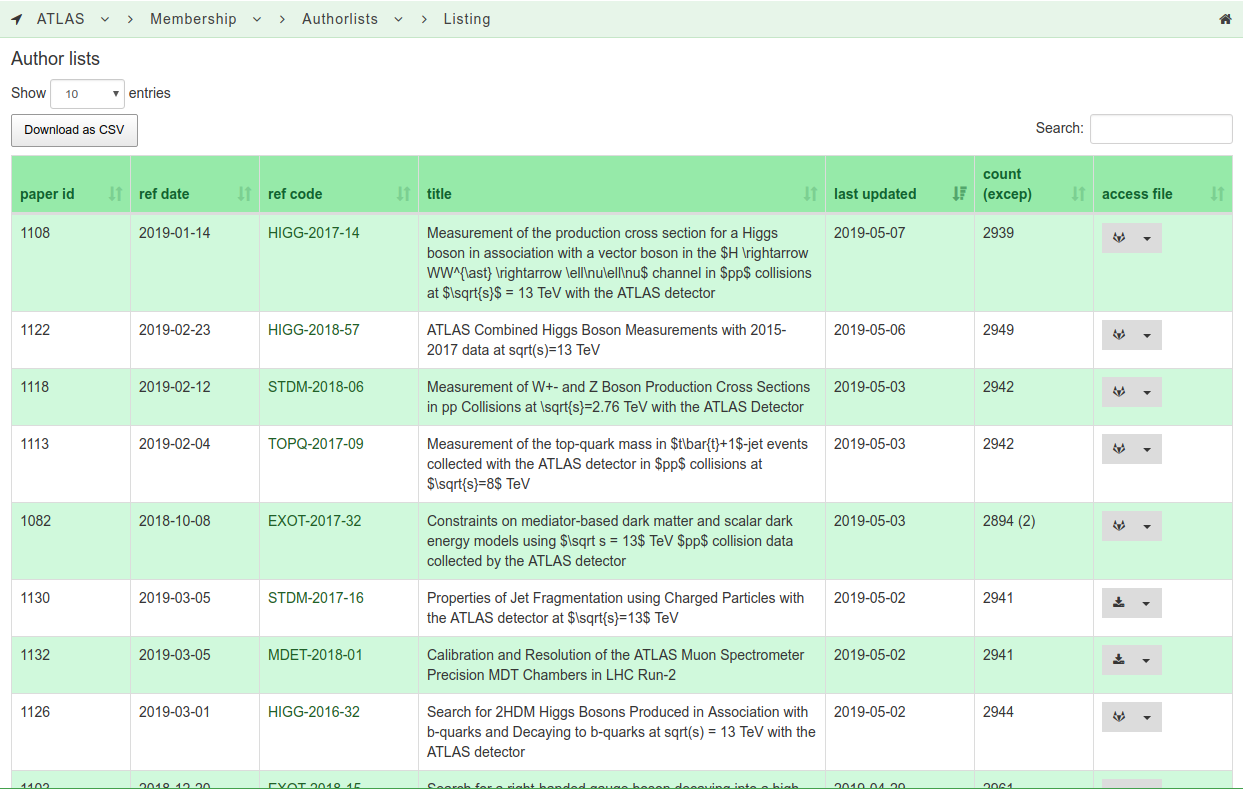
\includegraphics[width=0.9\textwidth]{figures/authorlist_interface.png}
  \caption{FENCE Authorlist interface. The five first in the list are GitLab projects.}
  \label{fig:authorlist_interface}
\end{figure}

\subsection{Main functionalities of the FENCE Author list user interface}
\label{sec:Main_functionalities_of_the_FENCE_Author_list_user_interface}

The FENCE Author list interface, Fig.~\ref{fig:authorlist_interface}, shows the complete set of author lists created for each ATLAS Paper which is published since 2009 or being submitted. They are easily filtered using the SEARCH box option. All the columns are self-explanatory; in the last column the dropdown menu gives access to the author list location, which can be distinguished by the icon: a download\textbf{ icon ()} means the files are stored in AFS and can be downloaded. A GitLab \textbf{icon ()} means the Paper and the files are located in a PO Gitlab repository. The author lists can be downloaded or displayed in Gitlab in different file formats (tex, xml, csv, pdf, cds) and structures (by country/institutes, or institutes only). 

\subsection{Proof checker functionalities}
\label{sec:Proof_checker_functionalities}
Once the author list is sent to the journal together with the publication, it’s time to check if the publisher correctly used the information provided by going through the journal pdf file sent to ATLAS Physics Office and comparing to the xml/tex file. This process, once done by hand, required the officer to verify if each author (~2800) and each institute (~200) is correctly reported and matched. 
For this purpose, a tool, the proof checker, was created to automatically poll the proof directories for new pdf documents uploaded. If it finds a document that has not been checked before, it starts the following process:

\begin{itemize}
\item Retrieves the information from the XML file created on Paper Submission Phase;
\item Extracts the text from the journal pdf file;
\item Parses the text from the pdf file, creating the target reference;
\item Compares the official reference obtained from the XML file with the target reference;
\item Creates a report with the differences found between the original and the target reference;
\item Links the report to the main report page, Fig.~\ref{fig:collaboration_proofs}.
\end{itemize}

\begin{figure}[ht!]
  \centering
  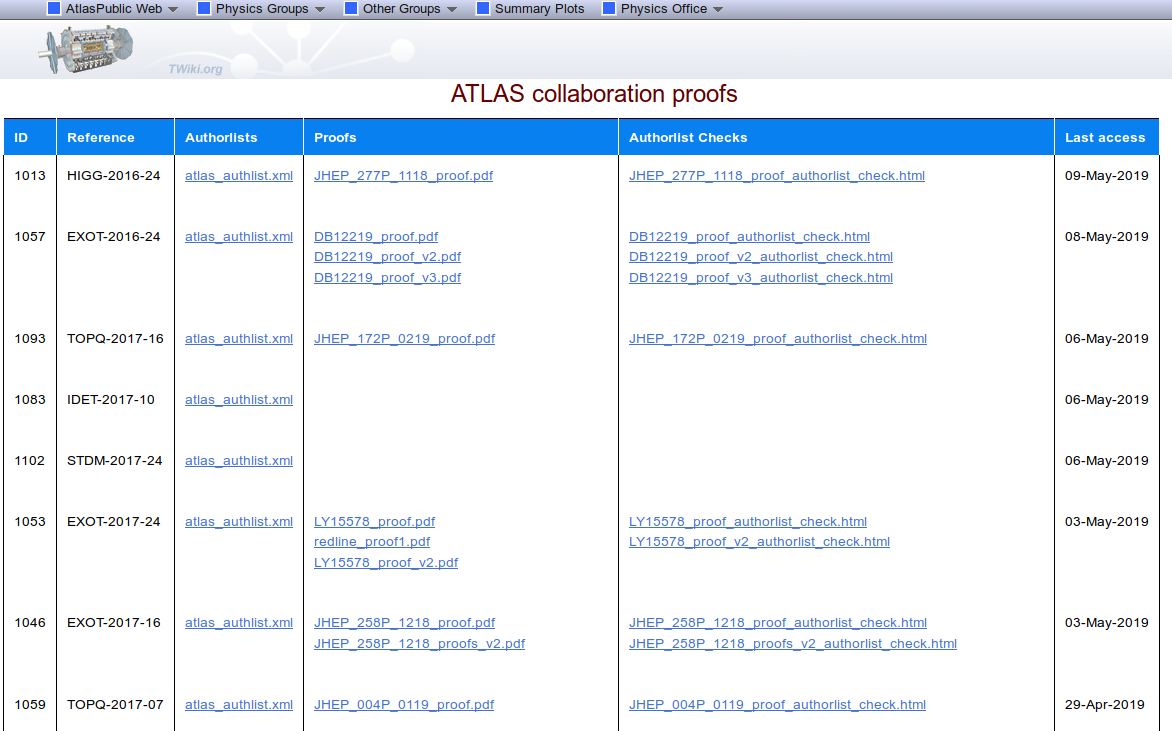
\includegraphics[width=0.9\textwidth]{figures/collaboration_proofs.png}
  \caption{Atlas collaboration proofs main page.}
  \label{fig:collaboration_proofs}
\end{figure}
The main difficulties in this process rely on extracting the content from the PDF file; the text is not easily retrieved for different reasons. 
One is that there are a lot of elements that have to be identified and ignored, such as row numbers, watermarks, footpages and headings. 
Another reason is that words extracted from a PDF file don’t follow a specific coding convention: other than ASCII characters can be output in many different ways; PDF can specify a predefined encoding to use, or provide a lookup table of differences to a predefined or built-in encoding; for fonts with non common latin characters, which is always the case for these kind of publications and content, special encodings are used and should be necessary to provide a ToUnicode table when semantic information about the characters has to be preserved. 
Also the proof checker has to pass through all the publication text and try to “understand” when the author list starts, when it ends, when the institute list starts and when it ends.
All this is made even more difficult due to the fact that different publishers have different layouts, and create different versions of PDF files, making all of the above problems not generic but often specific to themselves only.

After the target reference is created, the comparison looks for:

\begin{itemize}
\item Authors that seem to be missing from the PDF. Here, false positives are often due to characters encoding and spaces;
\item Authors with inconsistent punctuation. This section points out differences between original and target references authors’ first names punctuation to follow the rule X. or X.Y. or X.-Y. or X-Y. with no spaces at all.;
\item Institutes that seem missing from the PDF. Here false positives are often due to non standard characters which breaks the entry;
\item Institutes with close matches. All the entries that really look like the original but have some inconsistencies get in this group. Some publisher expands (or contracts) USA to United States of America, or there’s some new character which doesn’t break the institute entry but makes it so that there’s no perfect match, such as “Università” and “Universit` a”;
\item Mismatched authors. All the authors collaborate through one or more institutes. It is checked that the link between the author and the institute is consistent. This sometimes results as a false positive because it’s not always easy to extract from the pdf the index number of an institute, mainly because the text coming from the pdf file is often full of other elements such as line numbers of the document. For this reason an author originally assigned to institute number X, can result matched with target institute YX, because in the text extracted from the pdf the number X might be preceded by a Y line number; institute YX mostly doesn’t exist or eventually comes to be another institute;
\item Deceased authors. In two categories we show a list, often empty, of authors that we signed as deceased but the publication forgot to mark, or vice-versa. The results here are pretty reliable;
\item Missing founding agencies, or wrongly added by the publisher are checked.
\end{itemize}

In early 2019, due to some changes on CERN systems, the component written in PROLOG which run the comparison went out of service. This implied an urgent request for developing a new tool that could take care of this task. PROLOG is well known to take a different approach in a generic problem solving situation, where the expression of the problem is translated in a logic way instead of working directly on its resolution algorithm. But PROLOG is also a language difficult to maintain due to the fact that not many developers had ever a chance to work with it and its logic programming paradigm. That’s why python was chosen to accomplish this role.

The main issue was to find a way to get the best match among all the items of an array of institutes and authors because we can’t blindly rely on finding an author or institute in the same position of the sequence, and just compare author~1 on the xml file with author~1 in the pdf file and so on, as this is not always the case. For this purpose the concept of Levenshtein distance (\ref{sec:app16}) has been used, so that a weighted index of similarity could be obtained to “decide” what is matched with what, to then effectively start checking for anomalies.

At the end, a feature has been developed to help the script to evaluate as perfect matches some that wouldn’t otherwise. A list of “synonyms” is created for every entry, author or institute, to teach the proof checker to validate similar strings when the differences are due only to problems we have when decoding the text from the pdf file. So, for instance, if author \textbf{A. Filipčič} is not found in the target reference, but from the pdf entries we extracted an author with name \textbf{A. Filipž ciž c}, then, as it has been previously verified that in the pdf file the name appears as expected, the proof checker considers it a perfect match, and skips the problem. A very long list of false positives can be found in the report page as “skipped items”. The list of synonyms is updated manually, but a tool, the Synonym webpage (\ref{sec:Synonym_webpage}), has been created to allow users to update this list themselves.


\subsubsection{Proof checker synonyms}
\label{sec:Proof_checker_synonyms}
The comparison between PDF file (coming from the Journals) and the XML file (provided by FENCE author list interface) generates a lot of false positives as described in \ref{sec:Report_page}: special characters encoding can be different, countries sometimes are spelled differently, etc. To avoid having a huge list of these kind of false positives into the report page that can confuse the users, the new version of the proof checker includes a “synonyms” list that allows the comparison script to understand if the difference is a real error or another correct way to display the same information. An example of a working synonym is:
\begin{table}[ht!]
\centering
\begin{tabular}{|c|}
\hline
\textbf{Institute as stored into ATLAS DB \& XML file} \\
\hline
Physics Department, SUNY Albany, Albany NY, United States of America \\
\hline
\textbf{Institute as written on the journal’s author list} \\
\hline
Physics Department, SUNY Albany, Albany, New York, USA \\
\hline
\end{tabular}
\end{table}

These differences are acceptable, since the main information is correctly displayed and no real errors are found.

All the synonyms’ records are managed using a JSON file and splitted by institutes and authors (\ref{sec:app13} and \ref{sec:app14}). Having this as a JSON file allows the proof checker script to easily parse the records and understand if the faults must be marked as Journal errors or if they should be skipped.

\subsubsection{Synonym webpage}
\label{sec:Synonym_webpage}
To manage the list of proof checker’s synonyms ATLAS PO provides a webpage that allows users to search for an existing entry and manage the record synonyms. 
Searching for an institute, or author, will display the list of records that match the searching criteria (Fig.~\ref{fig:synonym_webpage}) and allows the users to edit the synonyms for the record.
Clicking the edit icon will show a new page section where users can insert their own known synonym for the record. This will be, after confirmation, added to the list of synonyms and will be taken into account by the next run of the proof checker.
\begin{figure}[ht!]
  \centering
  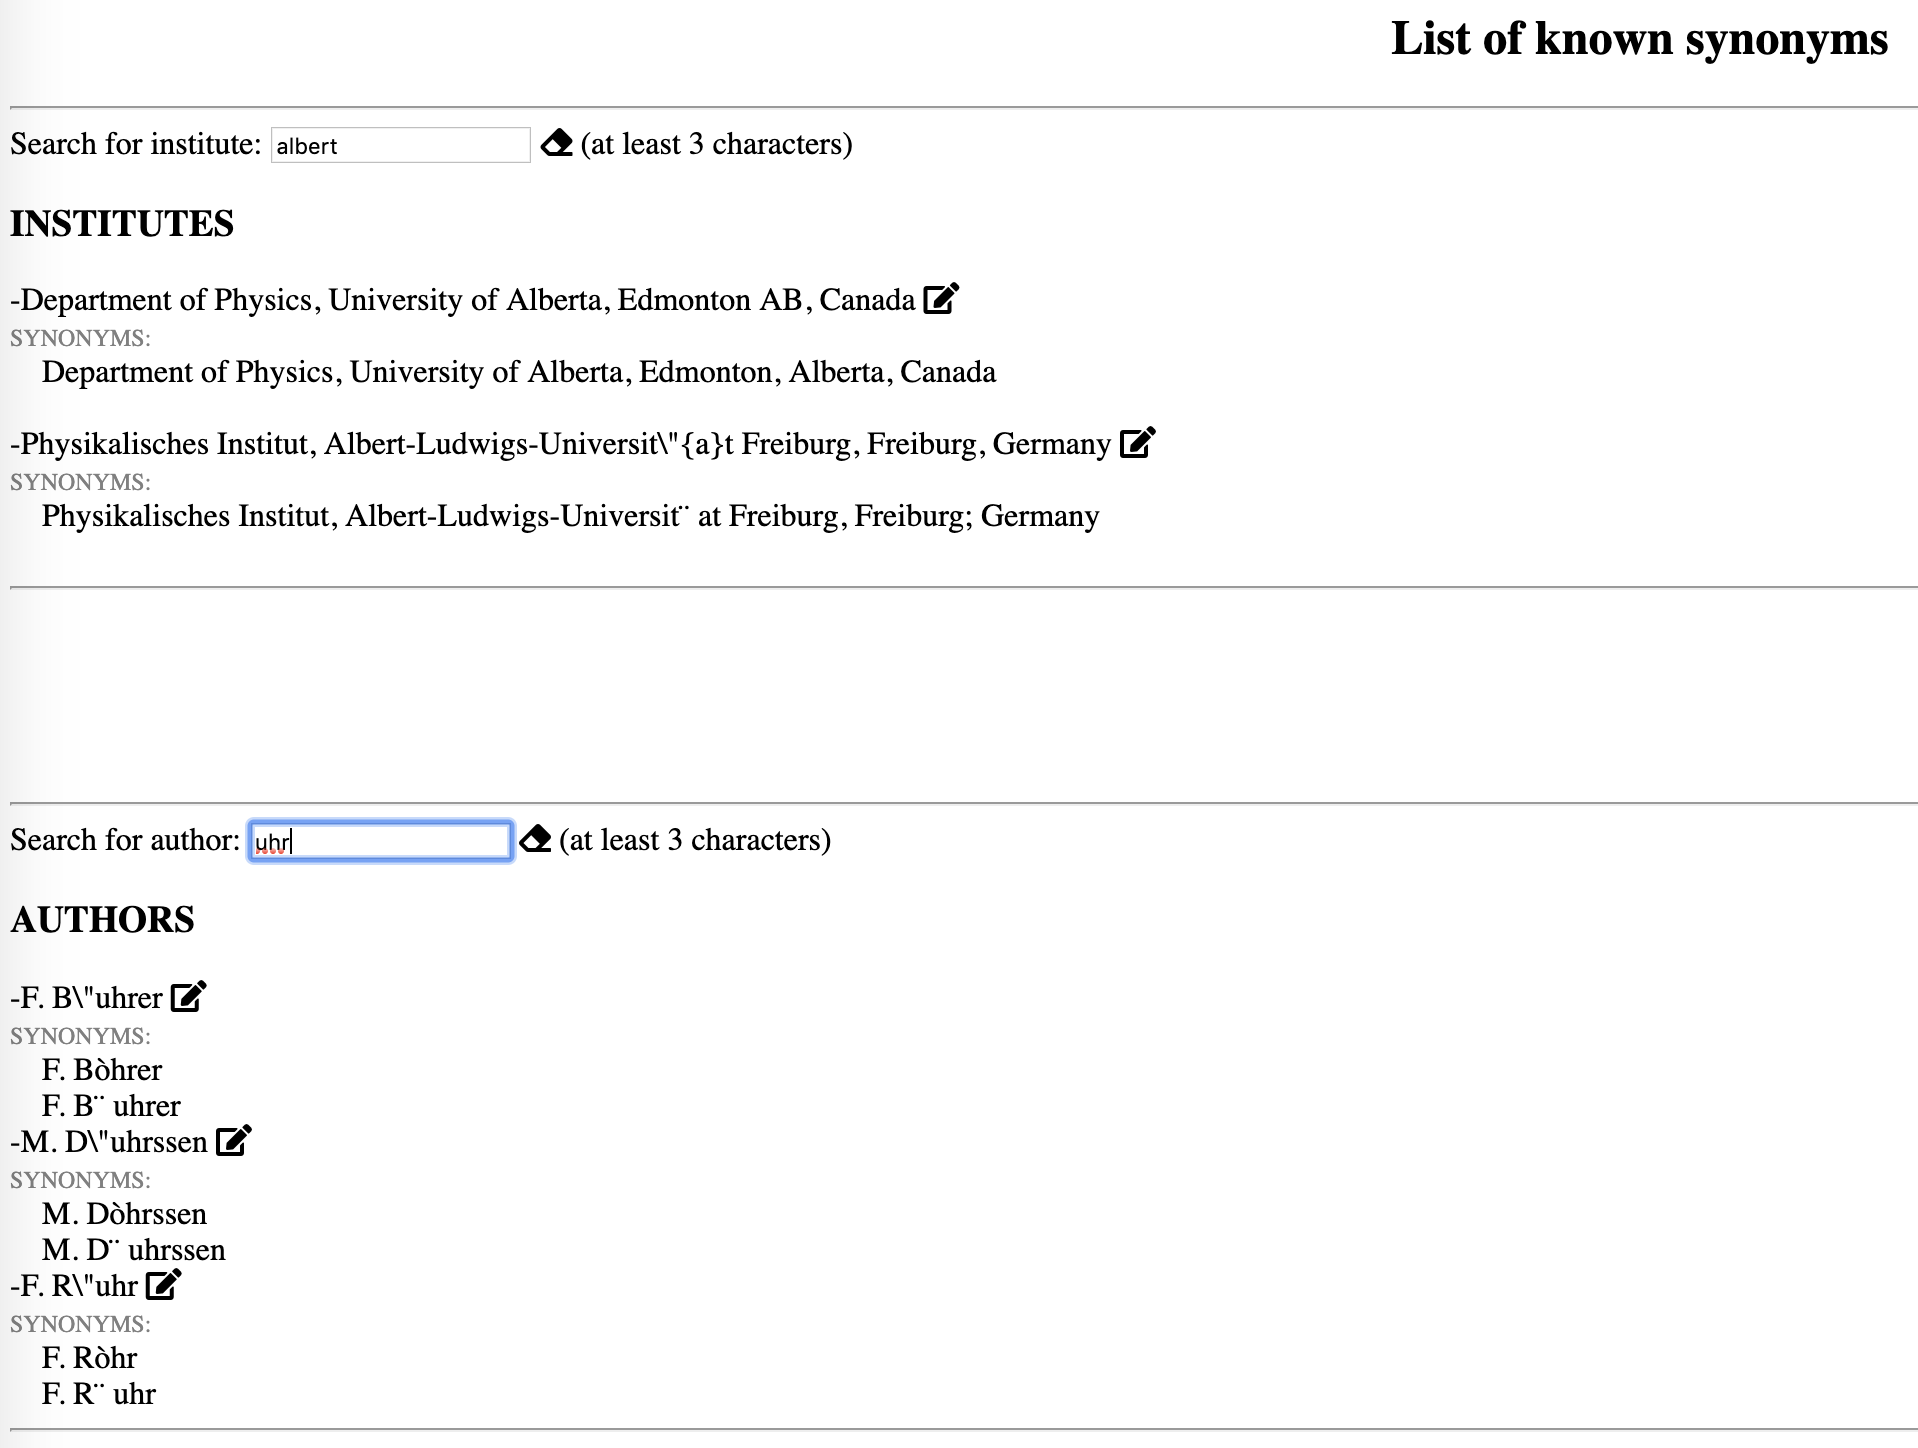
\includegraphics[width=0.9\textwidth]{figures/synonym_webpage.png}
  \caption{Proof checker synonyms’ webpage.}
  \label{fig:synonym_webpage}
\end{figure}

\subsubsection{Report page}
\label{sec:Report_page}
The proof checker provides a report after its run, one for each Paper and draft version. This report is provided and stored into a JSON file and must be parsed to show the report results into a human readable way. This is done by the proof$\_$report webpage (Fig.~\ref{fig:proof_report_webpage}).
On that report we can find all the paper information plus the real comparison results splitted by issue sections (see \ref{sec:app15}). The JSON file contains more information than what is displayed; this is done to allow the webpage to understand the correct way to show the huge amount of information and for future improvements. The webpage contains some “hidden” sections that are produced by the proof checker thanks to the known synonyms, and can be displayed by clicking on “Skipped +”. Here the page will show all the false positive results that the proof checker found on its comparison, but that are ignored thanks to the synonyms.
\begin{figure}[ht!]
  \centering
  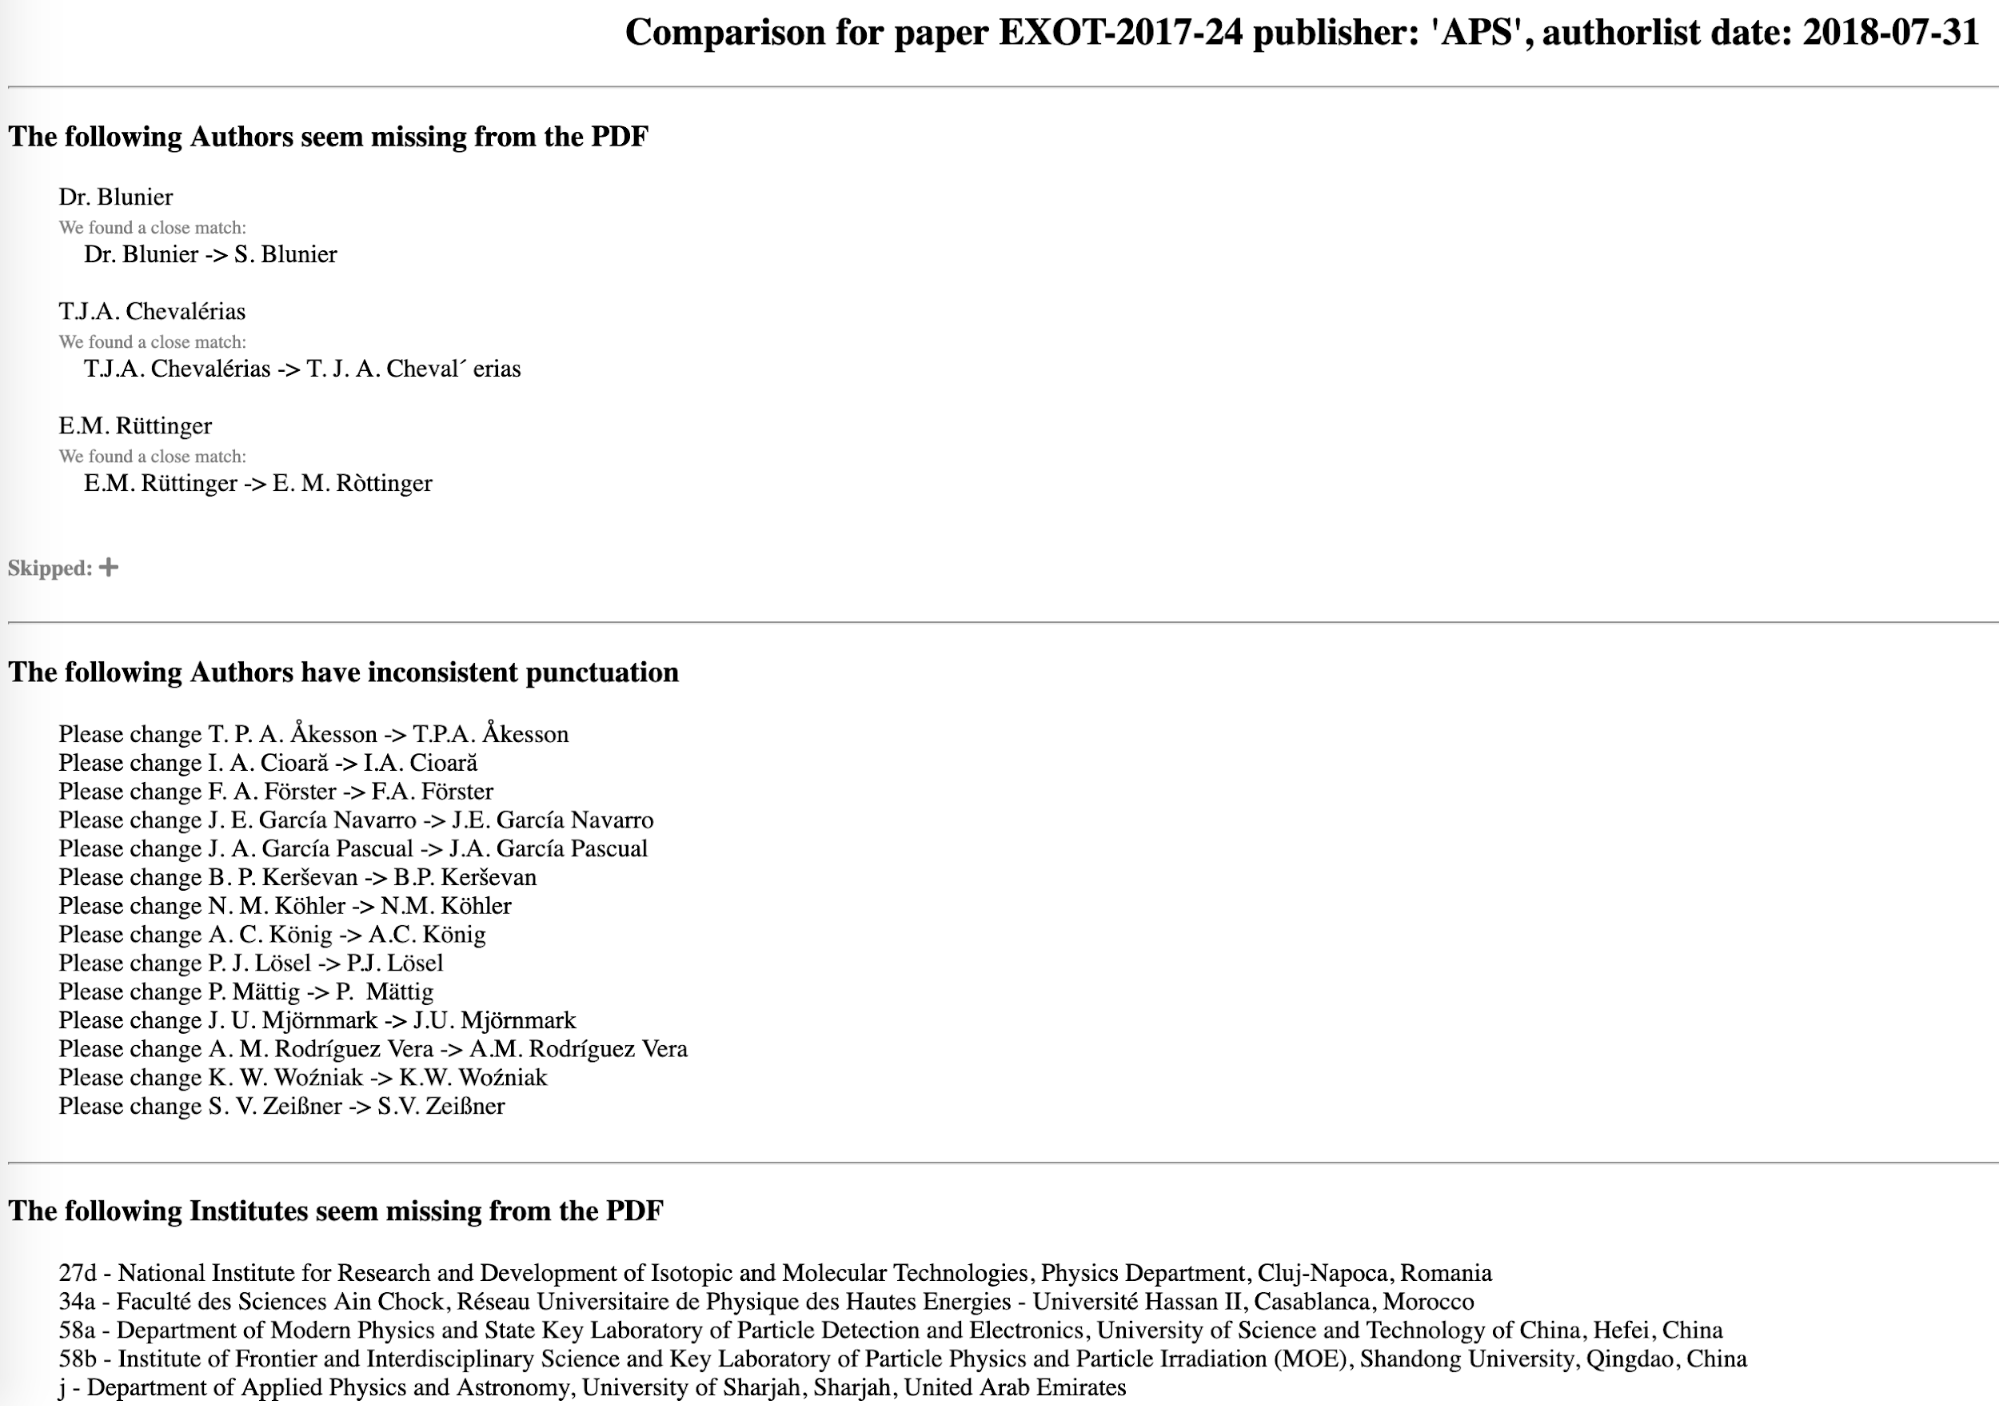
\includegraphics[width=0.9\textwidth]{figures/proof_report_webpage.png}
  \caption{Proof report webpage.}
  \label{fig:proof_report_webpage}
\end{figure}
The proof checker helps the Physics Office staff in a tedious task, but is way far from being a perfect tool. More than that, it will always need to be maintained and updated looking for new unexpected cases, changes on publication layouts, new conventions on the author lists and their format. A list of further improvements are in developers’ agenda, with the goal of having the user manually checking just a couple of dozens of cases instead of facing the list of hundreds of false positive they were used to until 2017.     

%-------------------------------------------------------------------------------

%-------------------------------------------------------------------------------
% 8 Handling the metadata
% !TEX root = ANA-GENR-2018-01-INT1.tex
% Turn off some chktex warnings.
% chktex-file 1 chktex-file 8 chktex-file 46

%------------------------------------------------------------------------------
\section{Handling the metadata}
\label{sec:Handling_the_metadata}
%------------------------------------------------------------------------------

%------------------------------------------------------------------------------
\subsection{Introduction}

The ATLAS database stores a lot of data and this must be retrieved and displayed in different ways through web pages.
The FENCE framework provides an API to retrieve those information.
A call to the API is allowed after a user authentication and provides the results in a JSON format.
This kind of information is easily parsed by most common programming languages and it is quite a standard for API results.
 
There are 3 main ways on how ATLAS PO provides web pages:

\begin{itemize}
\item standard HTML pages;
\item include files for TWiki pages;
\item FENCE webpages.
\end{itemize}

The first two options are running on ATLAS~PO Virtual Machine, which provides scripts, cronjobs or HTML pages to the users.
This Virtual Machine is directly connected to the FENCE framework to use its API and retrieve data, parse it and store into the EOS ATLAS file system.


%------------------------------------------------------------------------------
\subsection{ATLAS data in public pages}
\label{sec:ATLAS_data_in_public_pages}

FENCE also allows members who do not belong to ATLAS experiment to access some of the information stored in its database.
It provides different ways to retrieve and show the information: cron-job that runs on the ATLAS~PO Virtual Machine and extracts the data, parses it and shows it to the users.
 
An example where the data is retrieved using the FENCE API with a cron-job on the ATLAS~PO Virtual Machine is the ATLAS Map web page (\cref{fig:atlas_map_webpage}) where users can see on the map all the active institute members of the ATLAS collaboration.

\begin{figure}[htb]
  \centering
  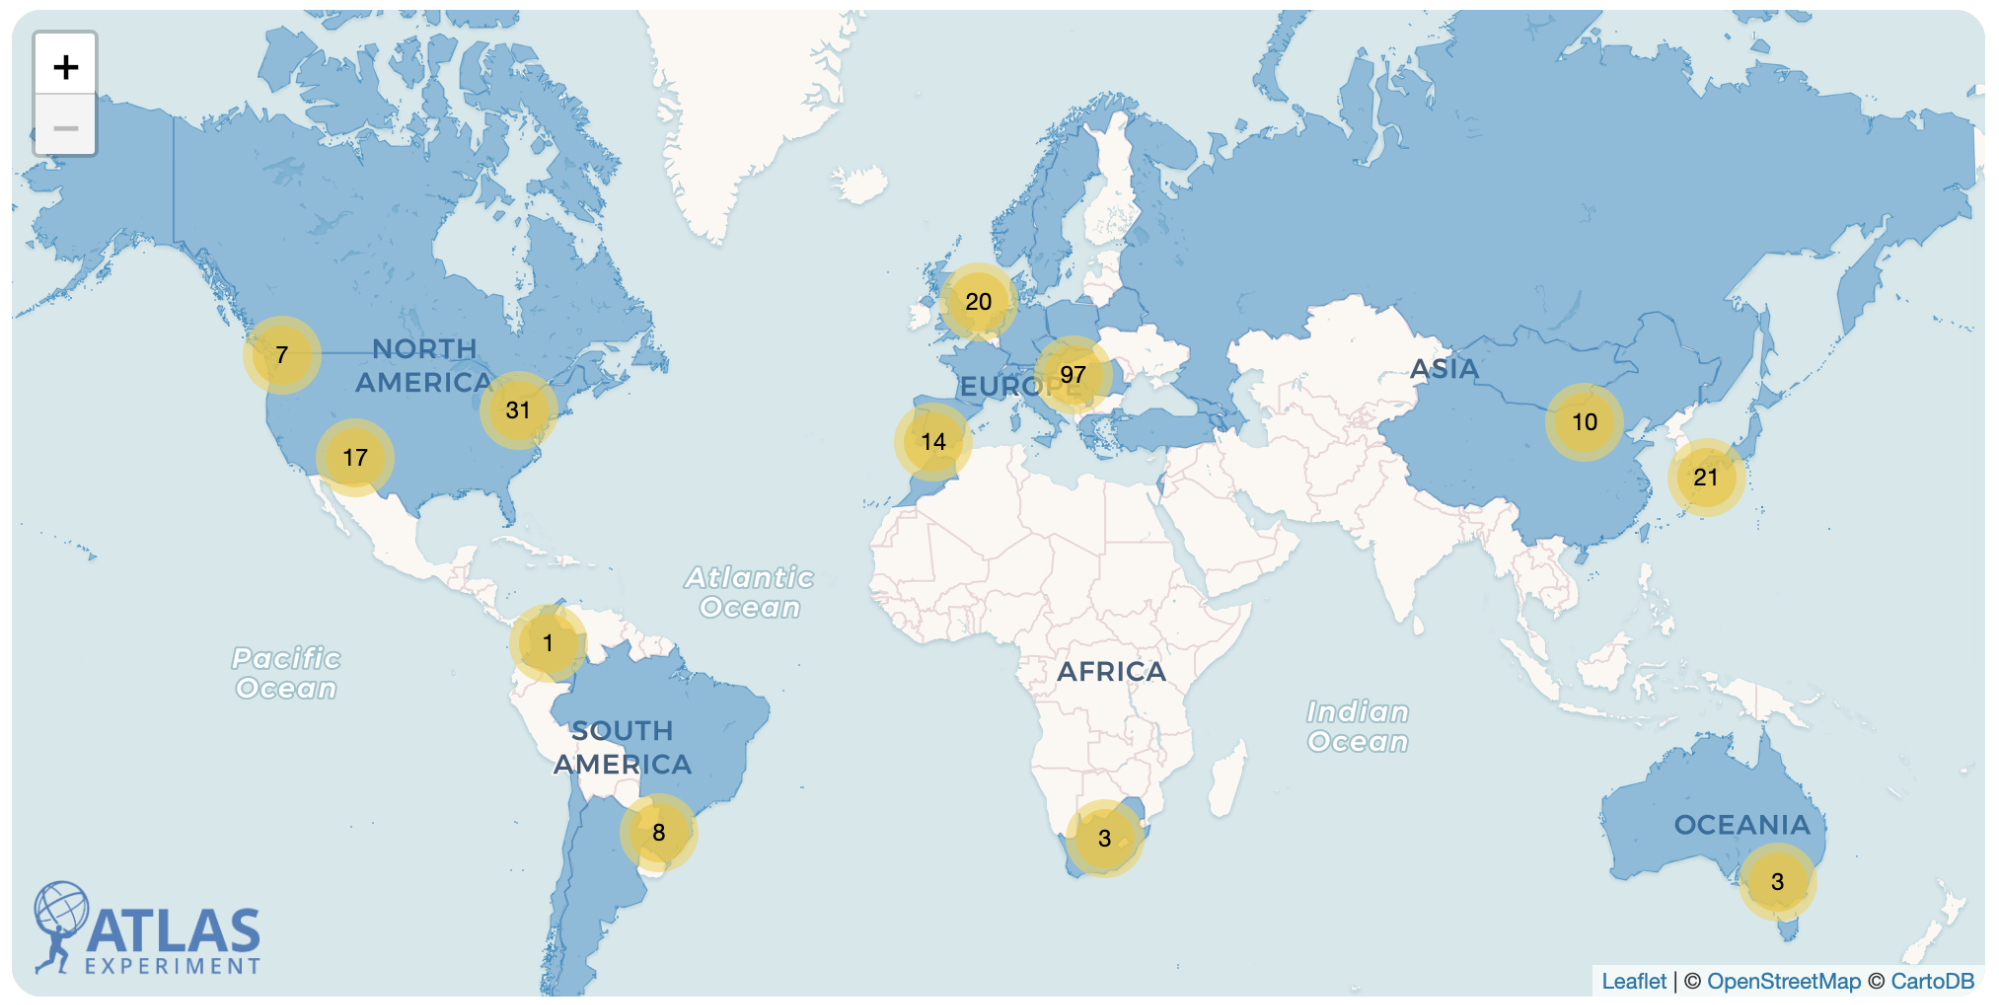
\includegraphics[width=0.9\textwidth]{atlas_map_webpage}
  \caption{The ATLAS map webpage.}
  \label{fig:atlas_map_webpage}
\end{figure}

This dynamic webpage filters the results to use only the active institutes.
This process is done on the ATLAS~PO Virtual Machine by a Python script,
which makes a request for the API, parses the results, and builds its own JSON file.
This file contains all the institutes information (name, country, links, coordinates, etc.) plus the layers to build the map.
Once the Python script builds the JSON file, the output is interpreted by the webpage, which takes care of displaying the layers and the markers for the institutes.


%------------------------------------------------------------------------------
\subsection{Data in TWiki pages}
\label{sec:Data_in_twiki_pages}

Displaying information on a TWiki page requires the use of TWiki \texttt{\%INCLUDE<path>} function.
This function allows to include the content of the \texttt{<path>} file and it will be interpreted by the TWiki page.
The content could be TWiki code or HTML code.
Having HTML code allows a more dynamic page to be created.
We can use javascript, jQuery and other web development tools to make the content more intuitive to the final user.
In this case the page will be loaded on-demand and the data will be displayed in real time thanks to the FENCE framework.

An example of an \texttt{include} using an HTML page which retrieves data using the FENCE API and displays it to the user into a TWiki page is the public results page (\cref{fig:public_twikipage}).
This page shows the full list of papers, CONF notes or PUB notes stored in the ATLAS database and managed by the FENCE framework.
It also allows users to filter results using the buttons on the top of the page.
This page loads ~1300 records with all the related information.
Retrieving all these records at once requires a lot of time.
To avoid this, the page initially loads only the first 10 records of each sections and makes the page available for user interaction,
then in the background it loads the other records.
This solution allows the loading process to run faster and avoids users having to wait for the complete data loading.

\begin{figure}[htb]
  \centering
  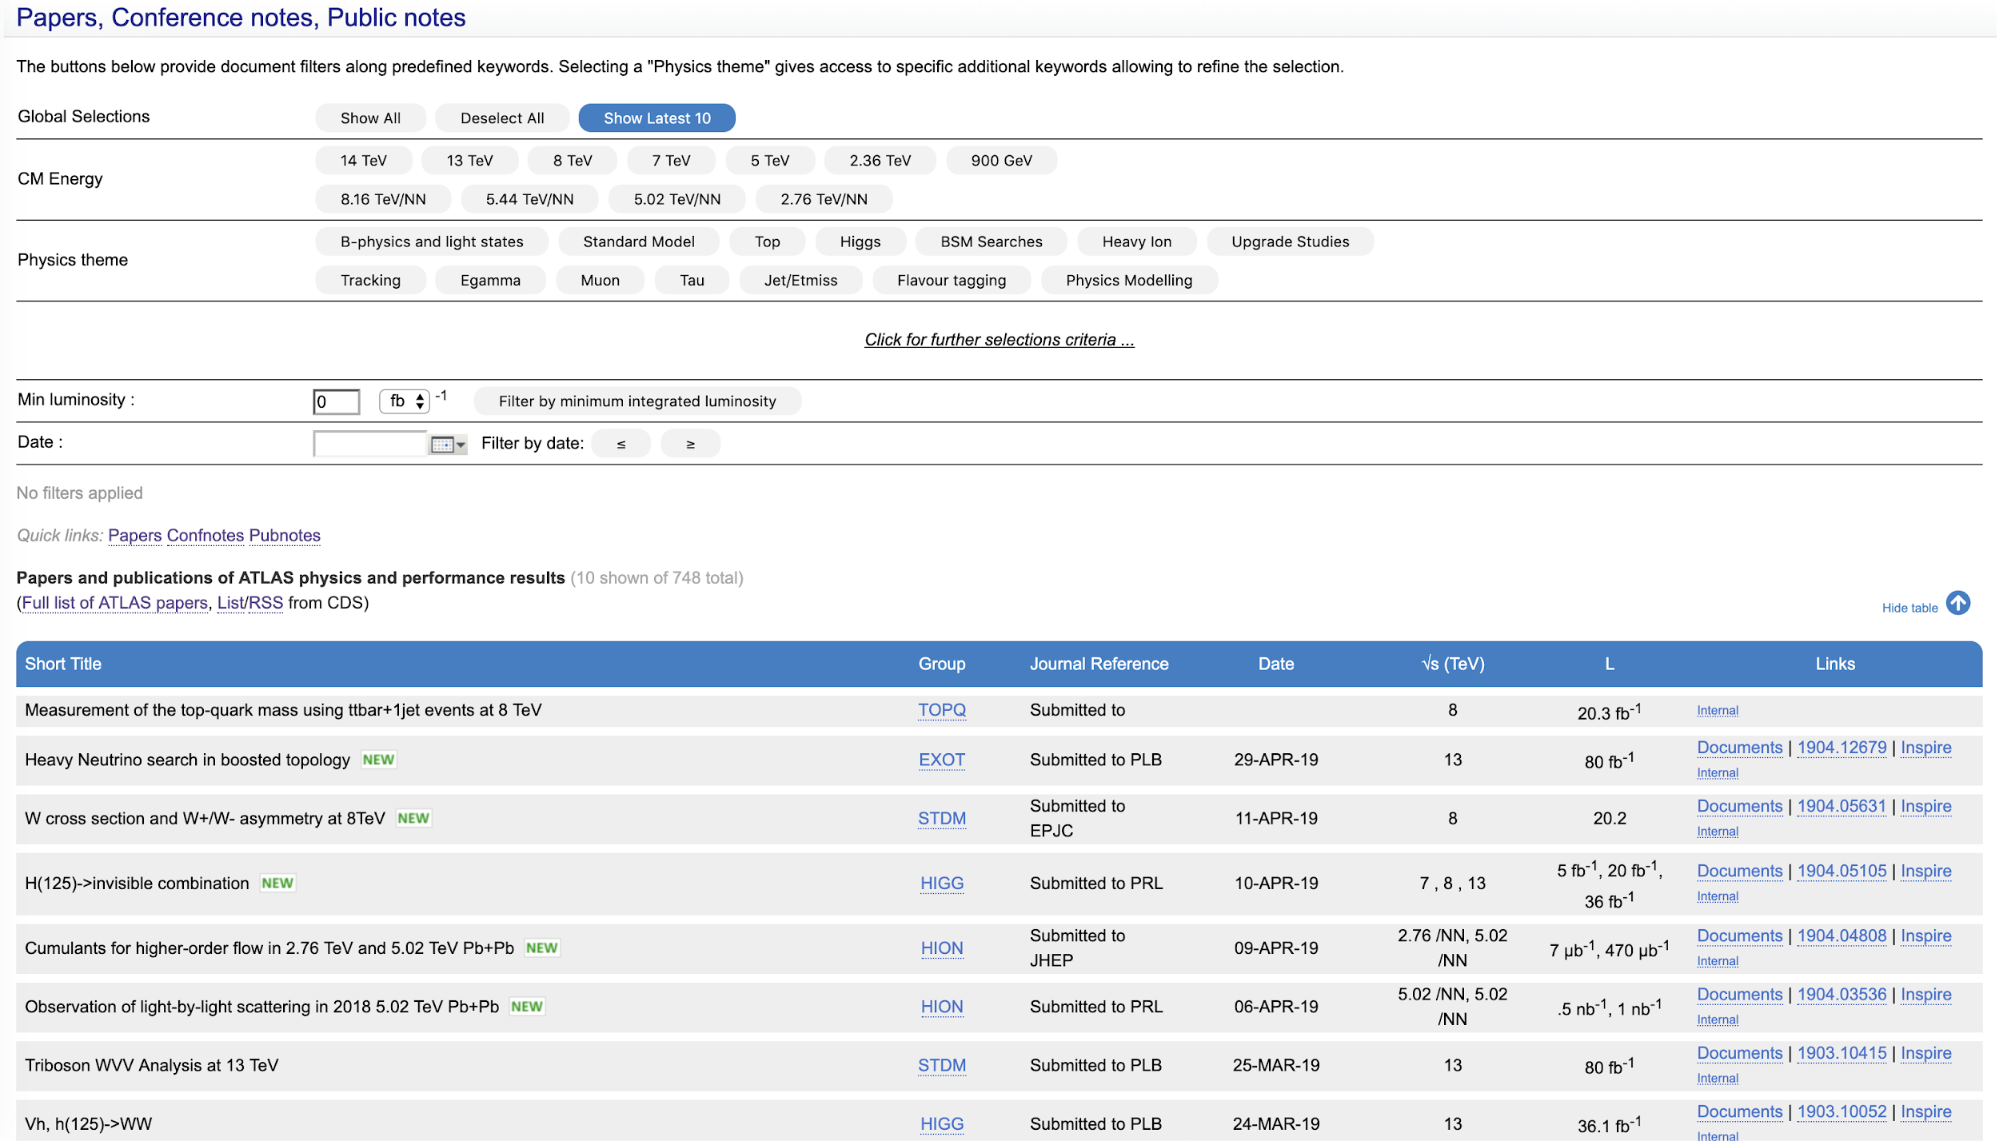
\includegraphics[width=0.9\textwidth]{public_twikipage}
  \caption{Public results TWiki page.}
  \label{fig:public_twikipage}
\end{figure}

\subsection{Data on FENCE public pages}
\label{sec:Data_on_FENCE_public_pages}

FENCE allows also to generate public web pages into its own framework instead of using other tools to retrieve and make the information into a human-readable format
This solution is the preferred one since the final data is displayed on call (real time information) and allows the use of all FENCE functionalities and classes,
that eases the building and maintenance of the web page.

%-------------------------------------------------------------------------------

%-------------------------------------------------------------------------------
% 9 Conclusion
% !TEX root = ANA-GENR-2018-01-INT1.tex
% Turn off some chktex warnings.
% chktex-file 1 chktex-file 8 chktex-file 46

%------------------------------------------------------------------------------
\section{Conclusion}
\label{sec:Conclusion}
%------------------------------------------------------------------------------

This documents summarises the framework that has been set up to support
the publication of documents by the ATLAS Collaboration.
While the emphasis is on papers published in refereed journals,
the system also supports internal documents and other public documents
such as Conference and Public notes.

The FENCE framework is used as a backbone of the whole setup
and is also used to interface the web-based tracking of the status of
an analysis with the documentation in \gitlab.
Extensive use is made of the Continuous Integration tools available in \gitlab
to ensure that documents can easily be submitted to arXiv and journals
as soon as they have been approved by the collaboration.

The system described in this document is now used to accompany
the whole of a physics analysis from the expression of interest of groups
that are interested in participating to the final journal publication.
It also includes the generation of the appropriate author list 
(including processing the proof-reading).

The tools are used by the whole of the collaboration and
minimise the amount of manual work required for repetitive procedures,
easing the workload of authors, editorial boards, management and the Physics Office.
At the same time all documents (and talks) connected to an analysis can now be accessed
from a central tool.

%-------------------------------------------------------------------------------

%-------------------------------------------------------------------------------
% Bibliography
\clearpage
\printbibliography
%-------------------------------------------------------------------------------

%-------------------------------------------------------------------------------
% Glossary
\clearpage
% !TEX root = ANA-GENR-2018-01-INT1.tex
% Turn off some chktex warnings.
% chktex-file 1 chktex-file 8 chktex-file 46

%------------------------------------------------------------------------------
\section{The FENCE project}%
\label{sec:The_FENCE_project}
%------------------------------------------------------------------------------

FENCE is an object-oriented \textit{PHP}~\cite{php} framework designed for the development of web applications.
Since it promotes reuse, similar features are implemented from predefined software components and, therefore, it speeds up the development process and reduces maintenance costs.
The FENCE software development process encompasses Software Engineering techniques such as requirements analysis, architecture, design, testing, deployment and maintenance in order to guarantee the quality of the software. Requirements are gathered and documented prior to the solution design and, this way, developers are able to propose broad solutions that can benefit the whole project. After any implementation is done, software tests are run to assure software correctness, robustness, extendibility and reusability.

%------------------------------------------------------------------------------
\subsection{FENCE main classes}%
\label{sec:FENCE_main_classes}

The FENCE framework is composed by a library of helper classes that are extensible program-code templates for creating objects, providing initial values and implementations of functions or methods.
Any new class can be coded and added to the framework, enlarging its scope, to then be reused in different systems.
One example is the \Class{GlanceSearch} class that provides methods to create search interfaces by adding only some lines of code and the specification of the search and results attributes through a configuration file.
The \Class{SuperSearch} class offers an advanced search interface, where the user can build logic queries with AND and OR operators.
The \Class{User} class supports the access control of the interfaces.
The \Class{Mailer} class can be used to send automatic emails.
Form inputs can be easily added using classes like \Class{TextInput}, \Class{DateInput} or \Class{MemberInput}, which provides a selection box with the list of all members of an experiment.

The FENCE \Class{Workflow} class is another example of feature that can be inherited by the systems that are implemented using the framework.
It can be applied to codify any process involving states and actions triggered while moving from a state to another.
This is used extensively by the ATLAS analysis systems, which are organised in phases, each one divided into several steps.
Each of those steps can record metadata in the ATLAS database, trigger an egroup~\cite{egroups} creation or update, an update on GitLab~\cite{gitlab}, send automatic emails and other tasks.


%------------------------------------------------------------------------------
\subsection{Configuration files in FENCE}%
\label{sec:Configuration_files_in_FENCE}

The FENCE framework proposal is based on configuration files that deploy content to be rendered on interfaces.\GSnote{}{Isn't this just the V part of MVC?}
The main goal of this infrastructure is to simplify many aspects of web systems requirements.
The configuration files are in JSON (JavaScript Object Notation), a lightweight format for storing and transporting data, and since those can be transformed in structured objects, developers can easily define a group of properties within specific contexts.
For instance, it is possible to set up which groups of users can have access to a certain interface.
Another benefit of using configuration files is that major classes, that have several arguments and environment parameters, can be instantiated in a cleaner way, with just a configuration file path as argument.
With that, developers feel encouraged to develop more generic and robust features, since they can be easily reused it in the future.

Along with the configuration file concept, additional utilities were developed to guarantee the feasibility of this idea.
\GSnote{One of these tools is the class \Class{JReader}, which parses a JSON input file, validates it and provides the JSON data to PHP code.}{How is this different from JSON Schema validation? I have a hard time understanding what it does better or different.}
Another one is the FENCE \Class{Content} class, which gets some default information from configuration file to handle common interface needs, such as access control, constants and rendering outline formats.

Most of the time, when a new interface is created using FENCE, the class that generates the particular content of this page is inheriting the \Class{Content} class.
At the same time, the \Class{Content} class, which has a configuration file path as argument, uses \Class{JReader} to validate and access the JSON properties.

\GSnote{}{Do you have a block-tree diagram that shows all of these relationships? Something like the one that gets generated when you run doxygen on C++ code}

%-------------------------------------------------------------------------------

%-------------------------------------------------------------------------------
\clearpage
\appendix
\part*{Appendix}
\addcontentsline{toc}{part}{Appendix}
%-------------------------------------------------------------------------------
\section*{Appendix 1}
\label{sec:app1}

\begin{lstlisting}
abstract class Graph
{
    abstract public function addNode(Node $node);
    abstract public function deleteNode(Node $node);
    abstract public function addEdge(Edge $edge);
    abstract public function deleteEdge(Edge $edge);
abstract public function clean();
}
\end{lstlisting}
\section*{Appendix 2}
\label{sec:app2}

\begin{lstlisting}
class Action
{
    protected $inputs;
    protected $outputs;
    protected $callback;

    public function __construct()
    {
        $this->inputs = array();
        $this->outputs = array();
    }

    public function setCallback($callback)
    {
        $this->callback = $callback;
    }

    public function getCallback()
    {
        return $this->callback;
    }

    public function setInputs($inputs)
    {
        $this->inputs = $inputs;
    }

    public function trigger()
    {
        $this->outputs = call_user_func_array($this->callback, $this->inputs);
    }

    public function getOutputs()
    {
        return $this->outputs;
    }
}
\end{lstlisting}
\section*{Appendix 3}
\label{sec:app3}

\begin{lstlisting}
{
    "label" : "Analysis definition after EOI meeting",
    "identifier" : "analysis_definition",
    "inputs" : [
        {
            "label": "Main physics aim",
            "name": "main_physics_aim",
            "about": "",
            "type": "textarea",
            "rules": {
                "maxlength": 500
            },
            "edit": {
                "usergroups": [
                    "GROUP_CONVENER",
                    "SUBGROUP_CONVENER",
                    "PROJECT_LEADER"
                ]
            }
        }
    ],
    "actions" : [
        {
            "next_state" : "analysis_coordinators_selection",
            "callback": {
                "class": "Atlas\\Analysis\\Analysis\\WorkflowActions",
                "method": "proceed"
            },
            "usergroups": [
                "GROUP_CONVENER",
                "SUBGROUP_CONVENER",
                "PROJECT_LEADER"
            ]
        }
    ],
    "notifications" : [
        {
            "template" : "EOI_MEETING_RESULTS",
            "task": "proceed",
            "deploy_on": "taskTriggers"
 },
        {
            "template" : "ANALYSIS_COORDINATOR_REQUEST",
            "task": "proceed",
            "deploy_on": "taskTriggers"
        }
    ]
}

\end{lstlisting}
\section*{Appendix 4}
\label{sec:app4}

\begin{lstlisting}
{
    "id" : "ANALYSIS_TEAM",
    "type" : "Analysis Team",
    "name" : "atlas-%ref_code%-analysis-team",
    "description" : "Analysis Team of %ref_code% (%short_title%)",
    "topic": "ATLAS PubComm",
    "admin_egroup" : "atlas-paperlists-admin",
    "members" : [
        {
            "type" : "field",
            "field" : "analysis_team"
        }
    ],
    "posting_exceptions" : [
        {
            "name" : "atlas-readaccess-current-physicists",
            "type" : "StaticEgroup"
        },
        {
            "name" : "service-cds-mail-robots",
            "type" : "StaticEgroup"
        }
    ]
}

\end{lstlisting}
\section*{Appendix 5}
\label{sec:app5}

\begin{lstlisting}
public function is_expert() 
{
    return $this->has_egroup("MailboxForwarding-atglance") || $this->has_egroup("fence-developers");
}

public function hasPermission($permission)
{
    return in_array($permission, $this->permissions);
}
\end{lstlisting}
\section*{Appendix 6}
\label{sec:app6}

\begin{lstlisting}
"pub_short_title": {
                "label": "Public short title",
                "sublabel": "Plain text, no LaTeX",
                "type": "textarea",
                "rules": {
                    "maxlength": 1000,
                    "character_not_allowed": ["\\", "$"]
                },
                "analysis_roles": [
                        "GROUP_CONVENER",
                        "SUBGROUP_CONVENER",
                        "PROJECT_LEADER"
                ]
            }
\end{lstlisting}

Taking the “GROUP$\_$CONVENER” role as an example, it uses the following method to grant permission to edit the Public short title field:

\begin{lstlisting}
public function is_subgroup_convener($publication_id = null)
{
        if ($publication_id === null) return false;
        foreach ($this->subgroup_convener_publications as $line => $row) {
                if (strpos($row['PUB_LIST'], strval($publication_id)) !== FALSE) return true;
        }
        return false;
}

\end{lstlisting}
\section*{Appendix 7}
\label{sec:app7}

\begin{lstlisting}
public function get($endPoint, $data = null)
{
    $this->init($endPoint, $data);
    return $this->exec();
}

public function post($endPoint, $data = null)
{
    return $this->execMethod('POST', $endPoint, $data);
}

private function delete($endPoint, $data = null)
{
    return $this->execMethod('DELETE', $endPoint, $data);
}

private function put($endPoint, $data = null)
{
    return $this->execMethod('PUT', $endPoint, $data);
}

\end{lstlisting}
\section*{Appendix 8}
\label{sec:app8}

\begin{lstlisting}
private function execMethod($method, $endPoint, $data = null)
{
    $this->init($endPoint);
    $this->setMethod($method);
    if ($data) {
        $this->setBodyData($data);
    }

    return $this->exec();
}

\end{lstlisting}
\section*{Appendix 9}
\label{sec:app9}

\begin{lstlisting}
public function createProject($project, $parameters = [])
{
    $name = $project;
    if ($project instanceof Project) {
        $name = $project->name();
    }

    \FENCE\Logger::debug("Creating project = {project}", ["project" => $project]);
    $payload = $this->post('projects', array_merge([
        'name' => $name
    ], $parameters));

    if (! isset($payload['id'])) {
        throw new Exception\ProjectAlreadyExistsException(
            json_encode($payload)
        );
    }

    return new Project($payload['id'], $payload);

}
\end{lstlisting}
\section*{Appendix 16}
\label{sec:app16}
Mathematically, the Levenshtein distance between two strings a,b of length |a| and |b| respectively is given by lev a,b(|a|,|b|) where
\begin{figure}[ht!]
  \centering
  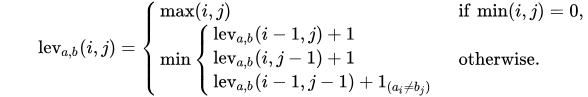
\includegraphics[width=0.9\textwidth]{figures/levenshtein.png}
  \label{fig:levenshtein}
\end{figure}
\par

Where 1(ai$\neq$ bj) is equal to 0 when ai = bj and equal to 1 otherwise, and leva,b(i,j) is the distance between the first i characters of a and the first j characters of b.

\section*{Appendix 10}
\label{sec:app10}

\begin{lstlisting}
<collaborationauthorlist
    xmlns:foaf="http://xmlns.com/foaf/0.1/"
    xmlns:cal="http://www.slac.stanford.edu/spires/hepnames/authors_xml/">
<cal:publicationReference>BPHY-2015-05</cal:publicationReference>
<cal:publicationReference></cal:publicationReference>
<cal:authorlistReferenceDate>2018-09-05</cal:authorlistReferenceDate>
<cal:creationDate>05-Dec-2018</cal:creationDate>

\end{lstlisting}
\section*{Appendix 11}
\label{sec:app11}

\begin{lstlisting}
<foaf:Organization id="o1">
    <cal:orgDomain>physsci.adelaide.edu.au/hep/</cal:orgDomain>
    <foaf:name>Department of Physics, University of Adelaide, Adelaide, Australia</foaf:name>
    <cal:orgName source="spiresICN">Adelaide U., Sch. Chem. Phys.</cal:orgName>
    <cal:orgName source="InstId">275</cal:orgName>
    <cal:orgName source="shortName">Adelaide</cal:orgName>
    <cal:orgStatus>member</cal:orgStatus>\
</foaf:Organization>

\end{lstlisting}
\section*{Appendix 12}
\label{sec:app12}

\begin{lstlisting}
<foaf:Person>
    <foaf:name>Georges Aad</foaf:name>
    <foaf:givenName>Georges</foaf:givenName>
    <foaf:familyName>Aad</foaf:familyName>
    <cal:authorNameNative></cal:authorNameNative>
    <cal:authorSuffix></cal:authorSuffix>
    <cal:authorStatus></cal:authorStatus>
    <cal:authorNamePaper>G. Aad</cal:authorNamePaper>
    <cal:authorCollaboration collaborationid="c1" position="" />
    <cal:authorAffiliations>
        <cal:authorAffiliation organizationid="o99" connection="" />
    </cal:authorAffiliations>
    <cal:authorids>
<cal:authorid source="INSPIRE">INSPIRE-00210391</cal:authorid>
        <cal:authorid source="ORCID">0000-0002-6665-4934</cal:authorid>
    </cal:authorids>
</foaf:Person>

\end{lstlisting}
\section*{Appendix 13}
\label{sec:app13}

\begin{lstlisting}
{
    "id": "2", 
    "original": "Department of Physics, University of Alberta, Edmonton AB, Canada"
    "synonyms": ["Department of Physics, University of Alberta, Edmonton, Alberta, Canada"],
}

\end{lstlisting}
\section*{Appendix 14}
\label{sec:app14}

\begin{lstlisting}
{
    "original": "F. B\\\"uhrer",
    "inspire": "INSPIRE-00356527", 
    "foafName": "Felix Buehrer"
    "synonyms": ["F. B\u00f2hrer", "F. B\u00a8 uhrer"], 
}

\end{lstlisting}
\section*{Appendix 15}
\label{sec:app15}

\begin{lstlisting}
{
    "ref_code": "EXOT-2017-24",
    "ref_date": "2018-07-31", 
    "creation_date": "29-Oct-2018",
    "publisher": "'APS'", 
    "document": "doc1053",
    "filename": "LY15578_proof_v2", 
    "authors_missing_skip": [...], 
    "authors_missing_list": [...],
    "authors_puntuation_list": [...]
    "institutes_missing_pdf_list": [...], 
    "institutes_missing_pdf_skip": [...], 
    "authors_mismatched_list": [...], 
    "authors_not_deceased_list": [...], 
    "authors_deceased_list": [...], 
    "institutes_close_matches_list": [...], 
    "founding_agencies_missing": [...],
    "founding_agencies_wrong": [...]
}
\end{lstlisting}

%-------------------------------------------------------------------------------

%In an ATLAS note, use the appendices to include all the technical details of your work that are relevant for the ATLAS Collaboration only (e.g.\ dataset details, software release used). This information should be printed after the Bibliography.

\end{document}
